\documentclass[10pt,journal,compsoc]{IEEEtran}
%
% If IEEEtran.cls has not been installed into the LaTeX system files,
% manually specify the path to it like:
% \documentclass[journal]{../sty/IEEEtran}

\usepackage{graphics} % for pdf, bitmapped graphics files
\usepackage{epsfig} % for postscript graphics files
%\usepackage{mathptmx} % assumes new font selection scheme installed
%\usepackage{times} % assumes new font selection scheme installed
\usepackage{amsmath} % assumes amsmath package installed
\usepackage{amssymb}  % assumes amsmath package installed
\usepackage{amsfonts} % assumes amsfonts package installed
\usepackage{epstopdf}
\usepackage{color}
\usepackage{comment}
\usepackage{algorithm}
\usepackage{bbding}
\usepackage{algorithmic}
\usepackage[mathscr]{eucal}
%\usepackage{algpseudocode}
\renewcommand{\algorithmicrequire}{\textbf{Input:}}  % Use Input in the format of Algorithm  
\renewcommand{\algorithmicensure}{\textbf{Output:}} % Use Output in the format of Algorithm  
\usepackage{mathrsfs}

%The self define macro

% *** PDF, URL AND HYPERLINK PACKAGES ***
%
%\usepackage{url}
% url.sty was written by Donald Arseneau. It provides better support for
% handling and breaking URLs. url.sty is already installed on most LaTeX
% systems. The latest version and documentation can be obtained at:
% http://www.ctan.org/pkg/url
% Basically, \url{my_url_here}.

\newtheorem{example}{Example}
\newtheorem{remark}{Remark}
\newtheorem{definition}{Definition}
\newtheorem{theorem}{Theorem}
\newtheorem{lemma}{Lemma}
\newtheorem{proof}{Proof}
\newtheorem{proposition}{\bf Proposition}
\newtheorem{problem}{Problem}


\newcommand{\tl}[1]{\textcolor{blue} {TL: #1 :TL} }
\newcommand{\ly}[1]{\textcolor{red} {LY: #1 :LY} }
\newcommand{\gs}[1]{\textcolor{green} {GS: #1 :GS} }

% *** Do not adjust lengths that control margins, column widths, etc. ***
% *** Do not use packages that alter fonts (such as pslatex).         ***
% There should be no need to do such things with IEEEtran.cls V1.6 and later.
% (Unless specifically asked to do so by the journal or conference you plan
% to submit to, of course. )

\def \BN {{\em BN}}
\def \BNs {{\em BNs}}
\def \BCN {{\em BCN}}
\def \BCNs {{\em BCNs}}
\def \STP {{\em STP}}
\def \Pe {{\tt Pe}}
\def \Pv {{\tt Pv}}
\def \Spe {{\tt Spe}}
\def \Ce {{\tt Ce}}
\def \Cv {{\tt Cv}}
\def \Ks {{\tt Kstep}}
\def \Ri {{\tt Rinput}}
\def \Lce {{\tt Lce}}
\def \Ded {{\tt Df}}
\def \BB {{\mathcal{B}}}
\newcommand \Input{{{$\mathsf{i}$}}}
\newcommand \State {{{$\mathsf{s}$}}}
\newcommand\Output {{{$\mathsf{o}$}}}
\newcommand  \Ustate {{{$\mathsf{S}$}}}

\newcommand{\rev}[1]{{\color{red}{#1}}}

% The figures path
\graphicspath{{figures/}}

% correct bad hyphenation here
\hyphenation{op-tical net-works semi-conduc-tor}

%=======================================================================================

\begin{document}

\title{Online Observability of \\ 
	Boolean Control Networks}
\author{Guisen~Wu,
	Liyun~Dai\Envelope,
	Zhiming~Liu,
	Taolue~Chen,
	Jun~Pang,
	Hongyang~Qu
\IEEEcompsocitemizethanks{\IEEEcompsocthanksitem
Guisen Wu, Liyun Dai and Zhiming Liu are with the School of Computer and Information Science, Southwest University
Chongqing, 400715 China. E-mail: \{wgs233,~dailiyun,~zhimingliu88\}@swu.edu.cn.
%
Taolue Chen is with the Department of Computer Science and Information Systems, Birkbeck, University of London. E-mail: taolue@dcs.bbk.ac.uk.
Jun Pang is with the Faculty of Science, Technology and Communication, University of Luxembourg. E-mail: jun.pang@uni.lu.
Hongyang Qu is with the Department of Automatic Control and Systems Engineering, University of Sheffield. E-mail: h.qu@sheffield.ac.uk.}
\thanks{Manuscript received April 19, 2005; revised August 26, 2015.}
}
 
\maketitle

%=======================================================================================


\begin{abstract}
Determining initial states of Boolean control networks (\BCNs)  is import in many applications. The existing  four types of BCNs' observability  have been proposed to study the initial state of \BCNs. However, all of them are offline observability, meaning that the input sequence is given before studying the \BCN's initial state and the input sequence  remains unchanged during the process of determining. In this paper, we present an online observability which is more powerful in determining the initial state of \BCNs. For online observability, we can derive and decide input sequence one by one based on the feedback from the outputs of the network in every time step. Moreover, we also propose determination algorithm for online observability.
%Moreover, we also propose determination algorithms and optimization brought by the online observability to further illustrate its advantages.
\end{abstract}

% Note that keywords are not normally used for peerreview papers.
\begin{IEEEkeywords}
Boolean control networks, observability, algorithms
\end{IEEEkeywords}


\IEEEpeerreviewmaketitle


% !Mode\dots ``TeX:UTF-8''
% !TEX root = ../root.tex
\section{Introction}
\label{sec:intro}
In 1960s, Nobel Prize winners Jacob and Monod found that  ``Any cell contains a number of `regulatory' genes that act as switches and can turn one another on and off. If genes can turn one another on and off, then you can have genetic circuits.'' \cite{Waldrop1992Complexity,cheng2009controllability}. Inspired by these Boolean-type actions in genetic circuits, the Boolean networks (\BNs) is firstly proposed by Kauffman \cite{Kauffman1968Metabolic} for modeling nonlinear and complex biological systems. Some general descriptions of the \BNs\ and its applications to biological systems can be found in Kauffman. Since then research interests in  \BNs\ have been motivated by the large number of natural and artificial systems. These natural and artificial systems describing variables display only two distinct configurations, and hence these describing variables take only two values, i.e., $\{0,1\}$  \cite{Akutsu2000Inferring, Shmulevich2002From, Faur2006Dynamical,Green2007The,Lou2010Multi,Fornasini2013Observability}.


When extenal regulation or perturbation is considered, \BNs\ are naturally extended to Boolean control networks (\BCNs) \cite{Ideker2001A}. The \BCNs\ can be used to solve various important realistic problems. For instance, \BCNs\ can be used to do structural and functional analysis of  signaling and regulatory networks \cite{Kaufman1999A, Klamt2006A} and \BCNs\ can be used for abduction based drug target discovery \cite{Biane2017Abduction}, furthermore \BCNs\ also can be used for pursuit evasion problems in polygonal environments \cite{Thunberg2011A}. For a better understanding, we make a brief introduction about how  \BCNs\ can be used to do structural and functional analysis of signaling and regulatory networks. Evolution has equipped cells with exquisite signaling systems which allow them to sense their environment. The immune system is a very important part of the signaling system, it can identify and eliminate foreign invading antigens. T-cells known as lymphocytes are a type of white blood cells, they play a central role in the immune system. T-cells can recognize protentially dangerous agents for cells and initiate an reaction against these agents. T-cells do so by T-cell receptors to detect foreign antigens bound to major histocompatiblity complex molecules, and then activate, through a signaling cascade, several transcription factors. As the interaction of the antigen-specific receptor of T-cells with its antigenic ligand can lead either to cell activation (1) or to a state of profound unresponsiveness (0). We would like to apply the \BCNs\ to study the T-cell receptor kinetics model better \cite{Kaufman1999A, Klamt2006A}. The network graph of the \BCN\ T-cell receptor kinetics model given in \cite{Klamt2006A} is shown in Fig.\ref{fig:6}. For more details, we refer the reader to read \cite{Klamt2006A}. Furthermore there is a approach to study large-scale \BCNs\ via network aggregations \cite{Zhang2017Observability}. However, in order to further improve the performance of systems, we make some optimizations about the definition of observability of \BCNs.
 \begin{figure}[thpb]
      \centering
      \framebox{\parbox{3in}{
		\centerline{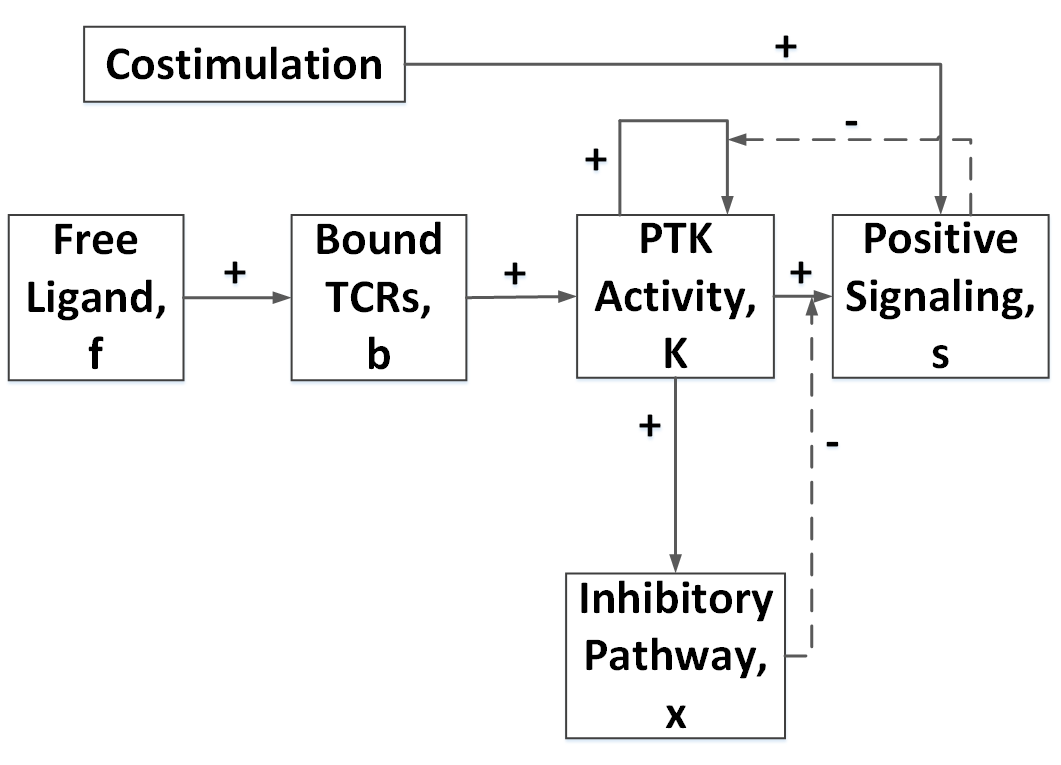
\includegraphics[scale=0.275]{figures/Fig6.png}}
	}}
      
      \caption{Network graph of the T-cell receptor kinetics model, where rectangles denote input nodes, the other nodes denote state nodes, particularly the nodes with shadows are chosen to be observed.}
      \label{fig:6}
  \end{figure}

As the wide application of \BCNs, it is important to research the control-theoretic problems of \BCNs. The study on control-theoretic problems of \BCNs\ can date back to 2007 \cite{Akutsu2007Control}. The work above also proves that the problem of determining the controllability of \BCNs\ is {\em NP}-hard in the number of nodes. Furthermore, it points out that ``One of the major goals of systems biology is to develop a control theory for complex biological systems.'' Since then, the study on control-theoretic problems in the areas of \BNs\ and \BCNs\ has drawn great attention \cite{cheng2009controllability, Zhao2010Input, Cheng2011Identification, Cheng2011Analysis,Fornasini2013Observability}. Besides controllability, observability is an another  basic control-theoretic problems and it also attract many attentions.  Among these studies, \emph{semi-tensor product} (STP) of matrices is one of useful tool to deal with  both \BNs\ and \BCNs\  related problems \cite{cheng2009controllability}.  Moreover,  \cite{cheng2009controllability} gives equivalent conditions for controllability of \BCNs\ and observability of controllable \BCNs. To date, there are four types of observability have been proposed. 

\begin{enumerate}
	\item The first type of observability proposed in 2009 \cite{cheng2009controllability} means that every initial state can be determined by an input sequence.
	
	\item 
	The second observability proposed in 2010 \cite{Zhao2010Input} stands that for every two distinct initial states, there exists an input sequence which can distinguish them, and this observability is determined in \cite{Li2015Controllability}.
	
	\item The third observability proposed in 2011 \cite{Cheng2011Identification} states that there is an input sequence that determines the initial state.
	
	\item  The fourth observability proposed in 2013 \cite{Fornasini2013Observability} is essentially the observability of linear control systems, i.e., every sufficient long input sequence can determine the initial state.
\end{enumerate}
 

%\tl{can you state the four types observability clearly and formally here?}

%\rev{****input s equence***}

In above mentioned definitions an input is not the value of an input-node, but it represents the values of all input-nodes of the \BCN\ on a time step. Therefore, an input can be seen as a vector of the values of all input-nodes of the \BCN\ on a time step. An input sequence consists of several inputs in sequential time steps.
     A output can also be seen as a vector of the values of all output-nodes of the \BCN\ on a time step. In every time step, there is a pair of input and output of \BCN. A output sequence also consists of several outputs in sequential time steps. In the following, we will list the informal definition of four offline  observabilities as well as the formal definition of four observabilities.% in the following pages.
 
The four  types of observability  have many nice properties that they can be used in some useful applications. However, all of four  types of observability of \BCNs\ are offline observabilities which means that they can not adjust the input sequence by observing the output sequence in the process of determining the initial state of \BCNs. Therefore, we propose the online observability that we can determine the initial state of \BCNs\ dynamically. In other words,  the online observability decides the input sequence in each time step by observing the out sequence. In the  online observability, we infer the possible  initial states set by observe the  first $k$ time steps output of \BCN. Through the  possible  initial states, we can choose one of input to refine the possible initial states set in the time step $k+1$. Repeat above procedure until the cardinality of initial states set turns into be one. We call this process is a dynamic process. 

\subsubsection*{Contribution}
Firstly, we propose the concept of the online observability of \BCNs. Compared with four existing observabilities, the online observability can help us to determine the initial state of some biological systems which can be checked at most once. Secondly, in addition to theoretical research, we also provide two algorithms to determine the online observability for \BCNs. Finally, we introduce some applications of the online observability of \BCNs. Including takes less observation costs, methods to find shortest path and approaches to avoid entering critical states when we use it to determine the initial state of \BCNs.  These applications will explain the advantages of online observability of \BCNs\ comparing with offline observabilities. %\rev{No important points}%\rev{***Compare with offline observabilities****} 
\subsubsection*{Structure}
The remainder of this paper is organized as follows. {\em Section \ref{sec:pre}} introduces necessary preliminaries about \BCNs, algebraic forms of \BCNs\ and the four existing kinds of observability of  \BCNs. {\em Section \ref{sec:online}} presents the definition of deduction function, $k$ steps determinability and online observability of \BCNs. {\em Section \ref{sec:deter}} presents how to determine the online observability of \BCNs\ by super tree and directed graph. {\em Section \ref{sec:app}} talks about some applications of the online observability of \BCNs. We also compare the online observability with offline observabilities in this section. {\em Section \ref{sec:con}} ends up  with the introduction of some future works.

%\tl{I will try to rewrite the intro.}

%==============================================================================================================
% !Mode\dots ``TeX:UTF-8''
% !TEX root = ../root.tex
\section{Preliminaries} 
\label{sec:pre}
In this section we introduce the definition of \BCNs\ and their algebraic form as well as the four existing kinds of observability of {\em BCNs}.



\subsection{Boolean Control Networks}

A Boolean control network can be described as a directed graph together with logical equations to describe the updating rules of the nodes of this directed graph, the definition of \BCN\ is as follows. 

\begin{definition}
(\cite{Ideker2001A}) A \BCN\ consists of input-nodes, state-nodes, output-nodes, and directed edges which connect nodes. A node in \BCN\ can take a logic value from $\{0,1\}$ at a discrete time $0, 1, 2,\ldots$ For one directed edge from a state-node $s_1$ (or an input-node $i_1$) to a state-node $s_2$ means that the logic value of $s_2$ at time step $t+1$ is affected by the value of $s_1$ (or $i_1$)  at time step $t$. For one directed edge from a state-node $s_1$ to a output-node $o_1$ means that the logic value of $o_1$ at time step $t$ is affected by the value of $s_1$  at time step $t$. 
\end{definition}


Note that one can only know that whether a node is affected by another node from the network graph. Different \BCNs\ may have the same structure, in order to determine a \BCN\ uniquely, logical equations are also needed to describe the specific updating rules of \BCNs.

 
 \begin{figure}[thpb]
      \centering
      \framebox{\parbox{3in}{
		\centerline{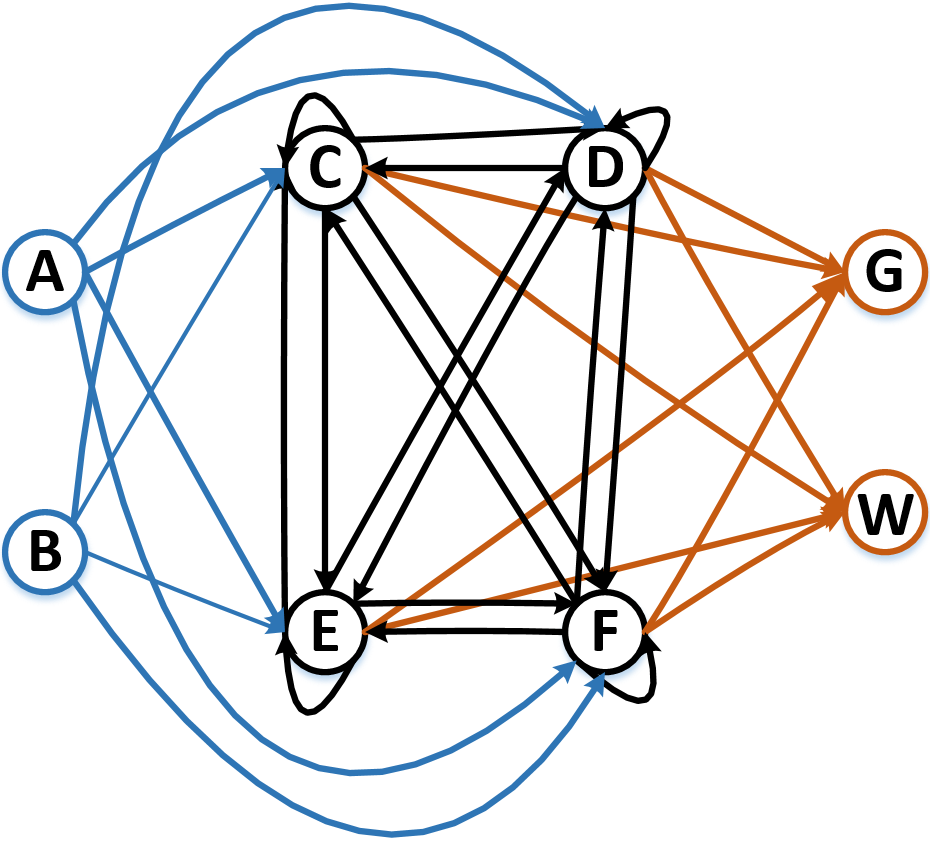
\includegraphics[scale=0.23]{figures/Fig1.png}}
	}}
      
      \caption{A Boolean control network with two input-nodes $A$ and $B$, four state-nodes $C$, $D$, $E$ and $F$, and two output-nodes $G$, $W$. We use blue, black and orange, to distinguish three kinds of nodes and three kinds of edges.}
      \label{fig:1}
  \end{figure}

To better illustrate the concept of {\em BCNs}, we give a simple example to describe it.

\begin{example}
	In Fig.\ref{fig:1} we have a \BCN\ with two input-nodes $A$ and $B$, four state-nodes $C$, $D$, $E$ and $F$, and two output-nodes $G$, $W$. The \BCN\ is shown in Fig.\ref{fig:1}, and the updating rules of this \BCN\ are described as truth table Fig.\ref{fig:2}. The reason why we use truth table to describe the updating rules of the \BCN\ is that this form of updating rules will be more convenient for \BCN\ to be converted into its aglebraic form. What's more, for instance, the updating rule of state-node $G$ is that,
	\[G(t)=C(t)\wedge \neg(\neg{D(t)}\wedge \neg E(t)\wedge \neg F(t))\]
	
	For convenience, we will use this example in the whole paper to explain various concepts we introduce.
  \begin{figure}[thpb]
      \centering
      \framebox{\parbox{3in}{
		\centerline{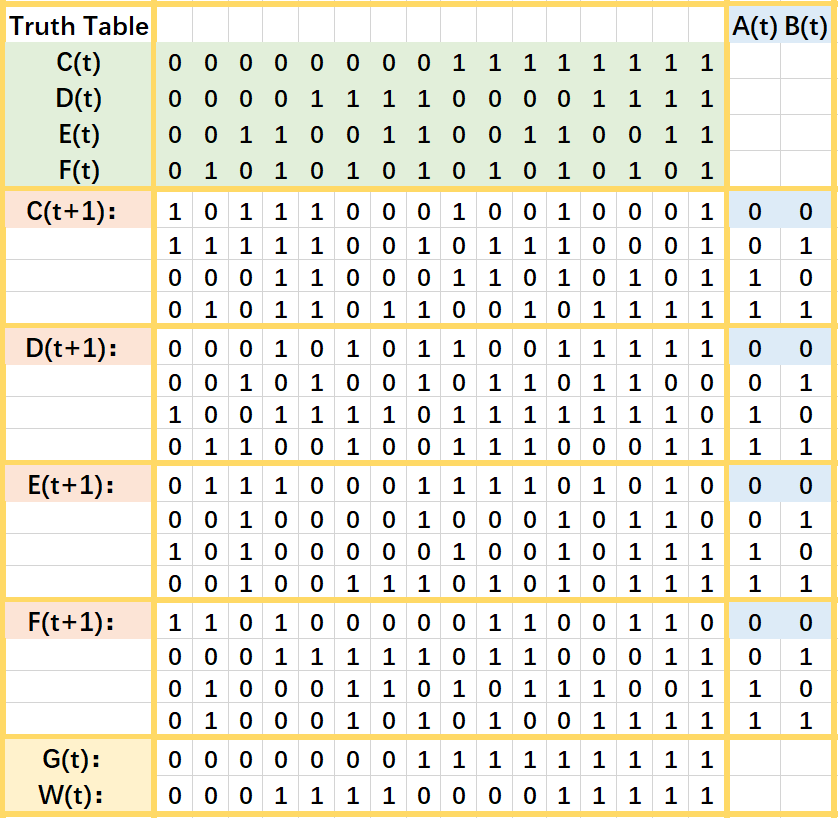
\includegraphics[scale=0.26]{figures/Fig2.png}}
	}}
      
      \caption{The truth table which describe the updating rules of the \BCN\ shown in {\em Fig.\ref{fig:1}}.}
      \label{fig:2}
   \end{figure}
\end{example}   


%==============================================================================================================
\subsection{The algebraic forms of \BCNs}
To better illustrate the concept of algebraic forms, in this paper, we investigate the \BCN\ in the following. And we suppose that this \BCN\ has $n$ state-nodes, $m$ input-nodes and $q$ output-nodes. Then the updating rules of the \BCN\ can be described as following formulas:
\begin{equation}
\begin{split}
s(t+1)=&f(i(t),s(t))\\
o(t)=&h(s(t))
\end{split}
\label{equ:1}
\end{equation}
$s(t)\in \mathbb{B}^n$ are state-nodes; $i(t)\in \mathbb{B}^m$ are input-nodes; $o(t)\in \mathbb{B}^q$ are output-nodes; $f:\mathbb{B}^{n+m}\mapsto \mathbb{B}^n$ and $h:\mathbb{B}^n\mapsto \mathbb{B}^q$ are logical functions that represent the updating rules of {\em BCNs}. Where $\mathbb{B}$ : the set $\{0,1\}$; $t=0,1,\ldots$ represents the discrete time. 

Therefore in the previously mentioned example, we have that $C(t), D(t), E(t), F(t)\in s(t)$; $A(t), B(t)\in i(t)$ and $G(t), W(t)\in o(t)$; $n=4$, $m=2$ and $q=2$; $f$ and $h$ are described in the truth table ({\em Fig.\ref{fig:2}}). 

Furthermore, the {\em STP} of matrices can be used to represent the algebraic forms of \BCNs\ \cite{cheng2009controllability}, the definition of {\em STP} is as follows.

\begin{definition}[STP] 
	\cite{Cheng2011Analysis} Let $X\in\mathbb{R}_{m\times n}$, $Y\in\mathbb{R}_{p\times q}$ and $\alpha=lcm(n,p)$ be the least common multiple of $n$ and $p$. The STP of $X$ and $Y$ is defined as \[X\ltimes Y=(X\otimes I_{\alpha/n})(Y\otimes I_{\alpha/p}),\] where $\otimes$ denotes the Kronecker product. 
\end{definition}

After introducing the definition of {\em STP} of matrices,  we introduce some related notations at first \cite{Zhang2016Observability}:
\begin{itemize}
  \item $\delta^i_n$: the $i$-th column of the identity matrix $I_n$;
  \item $\Delta_n$: the set $\{\delta^1_n,\ldots,\delta^n_n \}$; 
  \item $\delta_n \left[i_1,\ldots,i_s\right]$: $\left[\delta^{i_1}_n,\ldots,\delta^{i_s}_n\right]\left(i_1,\ldots,i_s\in\left\{1,2,\ldots,n\right\}\right)$ the logical matrix;
  \item  $L_{n\times s}$: the set of $n\times s$ logical matrices.
\end{itemize}


Using {\em STP} of matrices, the formula (\ref{equ:1}) can be quivalently represented in the following algebraic form:
\begin{equation}
\begin{split}
s(t+1)=&L\ltimes{i(t)}\ltimes{s(t)}\\
o(t)=&H\ltimes{s(t)}
\end{split}
\label{equ:2}
\end{equation}
where $s(t)\in\Delta_N$, $i(t)\in\Delta_M$, and  $o(t)\in\Delta_Q$ denote the states, inputs and outputs respectively the same as in formula {\em (\ref{equ:1})}, but $s(t)$, $i(t)$ and $o(t)$ in formula {\em (\ref{equ:2})} would be written in special vector forms; $L\in L_{N\times\left(NM\right)}$ and $H\in L_{Q\times N}$ denote the relation matrices; that $N=2^n$, $M=2^m$, and $Q=2^q$. Since {\em STP} keeps most properties of the conventional product \cite{Cheng2011Analysis}, the associative law, the distributive law, etc., we usually omit the symbol ``$\ltimes$'' hereinafter. For instance, the 
formula ``$s(t+1)=L\ltimes{i(t)}\ltimes{s(t)}$'' will be written as ``$s(t+1)=L{i(t)}{s(t)}$'' in the following pages.

To construct algebraic form (\ref{equ:2}) we give a mapping $\tau:\{0,1\}\mapsto \{\delta_2^1, \delta_2^2\}$ where $\tau(0)=\delta_2^2$, $\tau(1)= \delta_2^1$. 
%each logical value a vector form as: $1 \scriptsize{\sim} \delta_2^1$, $0 \scriptsize{\sim} \delta_2^2$. 
Therefore, the logical variable $A(t)$ takes value from these two vectors, i.e., $A(t)\in \{\delta_2^1, \delta_2^2\}$. Using the {\em STP} of matrices, we have 
\[i(t)=i_1(t){\ldots}i_m(t);\] 
\[s(t)=s_1(t){\ldots}s_n(t);\] 
\[o(t)=o_1(t){\ldots}o_q(t).\] 
And according to \cite{Cheng2003Semi}, each logical function $f_p$ of state-nodes can be found in the updating rules (\ref{equ:1}). The form of  $f_p$ as:
\[f_p(i_1(t),\ldots,i_m(t),s_1(t),\ldots,s_n(t))\] 
and there exists a structure matrix $L_p\in L_{2\times {NM}}$ such that
\begin{equation}
\begin{split}
\tau(f_p(i_1(t),\ldots,i_m(t),s_1(t),\ldots,s_n(t)))= L_pi(t)s(t)
\end{split}
\end{equation}
%where the left side of equation calculate the truth value and the  right side of equation calculate the vector in $\{\delta_2^1, \delta_2^2\}$. 
For state-nodes $s_1,\ldots,s_n$, we have $n$ logical matrices $L_1,\ldots,L_n$ for them, respectively. 
%We have that
%when\\
If for each state-node $s_p$ the logical matrix has its form
\[L_p=[\delta_2^{p_1},\ldots,\delta_2^{p_{NM}}],\] 
then we have that %for the set of all state-nodes $s(t)$ the logical matrix 
\[L=[\delta_N^{R_1},\ldots,\delta_N^{R_{NM}}]\]  where 
\[\delta_N^{R_1}=\delta_2^{1_1}\ldots\delta_2^{n_1};\ldots; \delta_N^{R_{NM}}=\delta_2^{1_{NM}}\ldots\delta_2^{n_{NM}}.\] 
%then 
By this relationship we can construct the $L$ for the algebraic forms of \BCNs. What's more we can also construct the logical matrix $H$ in the similar way. To better illustrate the concept of algebraic forms, we give a simple example to describe it.
\begin{example}
For instance, the \BCN\ whose structure is depicted in Fig.\ref{fig:1}, and the updating rules of this \BCN\ is described as truth table in Fig.\ref{fig:2}. We have that the updating rules of this \BCN\ can be represented with the algebraic form:
\begin{equation}
\begin{split}
s(t+1) =&\delta_{16}[\alpha]i(t)s(t)\\
o(t) =&\delta_4[\beta]s(t)\\
\end{split}
\label{equ:4}
\end{equation}
where $\alpha=\{10,4,11,16,9,5,1, 7,15,2,3,12,7,6,8,13,8,9,\\15,10,14,4,3,16,1,14,12,13,5,7,2,6,7,2,3,13,13,9,5,1,\\16,13 ,6,14,11,10,4,15,1,14 ,7,6,9 ,8,11,12,5,5,13,3,10,\\12,16,16\}$, $\beta=\{1,1,1,2,2,2,2,3,3,3,3,4,4,4,4,4\}$, $t\in \mathbb{N}$, $s\in \Delta_{16}$, $i\in \Delta_4$ and $o\in \Delta_4$.
\end{example}   
\subsection{Four existing observability of \BCNs}
In this subsection we introduce four existing kinds of observability of \BCNs. Let $\Delta_N$, $\Delta_M$, $\Delta_Q$ be three alphabets, for all $s_0\in \Delta_N$ and all $p\in \mathbb{Z}_+$; $\infty$ is the infinite natural numbers. In order to introduce four existing kinds of observability of {\em BCNs}, we define the mappings \cite{Zhang2016Observability}:
\begin{equation}
\begin{split}
L^p_{s_0} &: (\Delta_M)^p\mapsto(\Delta_N)^p, i_0\ldots i_{p-1} \mapsto s_1 \ldots\, s_p\\
L^{\infty}_{s_0} &: (\Delta_M)^{\infty}\mapsto(\Delta_N)^{\infty}, i_0 i_1 \ldots  \mapsto s_1 s_2 \ldots
\end{split}
\end{equation}
\begin{equation}
\begin{split}
(HL)^p_{s_0} &: (\Delta_M)^p\mapsto(\Delta_Q)^p, i_0\ldots i_{p-1} \mapsto o_1\ldots\, o_p\\
(HL)^{\infty}_{s_0} &: (\Delta_M)^{\infty}\mapsto(\Delta_Q)^{\infty}, i_0 i_1 \ldots  \mapsto o_1 o_2\ldots
\end{split}
\end{equation}

For all  $p\in \mathbb{Z}_+$, all $I=i_1 \ldots i_p \in(\Delta_M)^p$, and all $1\ge p \ge j \ge |I|$, we use I[p,j] to denote the word $i_p \ldots i_j$ as a input sequence. Then four existing kinds of observability of BCNs can be define as: 
\begin{definition}
The first kind of observability is that, \BCN\ is called observable, if for every initial state $s_0 \in \Delta_N$, there exists an input sequence $I\in(\Delta_M)^p$ for some $p\in \mathbb{Z}_+$ such that for all states $s_0\neq {s'}_0\in \Delta_N$, $Hs_0=H{s'}_0$ implies $(HL)^p_{s_0}(I)\neq (HL)^p_{{s'}_0}(I)$ \cite{cheng2009controllability}.
\end{definition}

Hence the first observability means that if a \BCN\ is observable then every initial state of the \BCN\ can be determined by an input sequence. But we can only use the corresponding input sequence of a state to check whether this state is the initial state of the {\em BCN} or not.
\begin{definition}
	The second kind of observability is that a \BCN\ is called observable if for any distinct states $s_0$, ${s'}_0 \in \Delta_N$, there exists an input sequence $I\in(\Delta_M)^p$ for some $p\in \mathbb{Z}_+$, such that $Hs_0=H{s'}_0$ implies $(HL)^p_{s_0}(I)\neq (HL)^p_{{s'}_0}(I)$ \cite{Zhao2010Input}.
\end{definition}

The second observability means that a \BCN\ is called observable if for every two distinct initial states of the {\em BCN}, there exists an input sequence which can distinguish them. 
\begin{definition}
	The third kind of observability is that, a \BCN\ is called observable, if there exists an input sequence $I\in(\Delta_M)^p$ for some $p\in \mathbb{Z}_+$, such that for any distinct states $s_0$, ${s'}_0 \in \Delta_N$, $Hs_0=H{s'}_0$ implies $(HL)^p_{s_0}(I)\neq (HL)^p_{{s'}_0}(I)$ \cite{Cheng2011Identification}.
\end{definition}

The third observability means that a \BCN\ is called observable if there is an input sequence that determines the initial state of the {\em BCN}.
\begin{definition}
	The fourth kind of observability is that, \BCN\ is called observable, if for any distinct states $s_0$, ${s'}_0 \in \Delta_N$, for any input sequence $I\in(\Delta_M)^{\infty}$, $Hs_0=H{s'}_0$ implies $(HL)^{\infty}_{s_0}(I)\neq (HL)^{\infty}_{{s'}_0}(I)$ \cite{Fornasini2013Observability}.
\end{definition}

The fourth observability means that a \BCN\ is called observable if every sufficient long input sequence can determine the initial state of the \BCN.

Then from the definitions of  four existing kinds of observability, we know that \cite{Zhang2016Observability}:
\begin{itemize}
  \item the first one implies the second one;
  \item the third one implies the second one and first one;
  \item the fourth one implies the third one, second one and first one.
\end{itemize} 
%, when we don't presuppose the initial state of {\em BCNs}
 
We can not use the first one and second one to determine the initial state of \BCNs\ which can be checked at most once. For example, in the first kind observability we need to assume the initial state of a \BCN, and then check it by corresponding input sequence of this state. If the state we assume is correct, then we can determine the initial state. But if the the assumption is not correct, we can not determine the initial state of the \BCN. Therefore we need to check several test cases (with the same initial state) of this \BCN\ untill we can determine the initial state of it. However we can use the third existing observability and fourth existing observability to determine the initial state of \BCNs\ through one test case. And we need not to presuppose the initial state of \BCNs\ when we use the third observability and fourth observability. But the requirements for \BCNs\ are very harsh when we use the third observability and fourth observability.
 
In some biological systems, the initial states of them can be checked at most once, i.e., we have only one test case for them. Therefore, we can not use the first observability and second observability to determine the initial states of them in real time. And in some biological systems, it would takes many costs to check these biological systems. Hence we will spend a lot of overhead to determine the initial states of them by the first observability and second observability. Furthermore, we also can not use the third observability and fourth observability to determine the initial states of some biological systems when they can not satify the requirements of the third observability and fourth observability. With these disadvantages of four existing observabilities, we propose the online observability of \BCNs\ to solve this problem.
 \subsubsection*{Problem}
Finding the necessary and sufficient condition of determine the initial state of \BCNs\ in real time.
% !Mode\dots ``TeX:UTF-8''
% !TEX root = ../root.tex
\section{The online observability of \BCNs}
\label{sec:online}
In this paper we propose the online observability, the informal definition of it is as follows. 

\begin{definition}
	A \BCN\ is called online observable, if every initial state $s_0 \in \Delta_N$ can be determined in one time by dynamically deciding input sequence and observing output sequence at every step without presupposing the  initial state of \BCN. And this process can be accomplished in finite steps.
\end{definition}

%\tl{maybe I did not understand this, but I think you are confusing two things: the observability and the algorithm (approach) to determine the initial state. It seems to me that you are describing a new approach (the online approach), but does this change the observability? if yes, how? Is this a stronger notion or a weaker notion or incomparable?}

In this section, firstly we present the definition of deduce function, secondly we present the definition of $K$ steps deterministic. We take them as the preparations for defining online observability. Finally, we give the formal definition of online observability of \BCNs. 
\subsection{Deduce function}
Different from four existing types, the observability we propose can determine the initial state online. Because in the process of determining the initial state every input of the input sequence is decided by the output we observe at every time step. At the beginning, we can observe the output of \BCNs, so that we can infer the possible values of state-nodes and treat them as possible states set $S_0$. Then as we can know the possible states set, we need to decide the input $i_0$. The input $i_0$ will make sure any different possible states $s_i, s_j \in S_0$ will not turn into the same state after affected by input $Ls_i i_0\neq Ls_j i_0$. After decided input, we can observe the new output, and then we can infer the new possible states set. The cardinal number of possible states set after we inputted will not lager than the cardinal number of possible states set before we input. If the cardinal number of possible states set turn into be $1$ then we can determine the state and the initial state of {\em BCN}. To simulate this deduction process, we give the definition of deduce function that.
\begin{definition}[Deduce Function] The deduce function can be defined as $D\left(S, I, O\right)$. Based on deduction process, we have for any \[s_i(t+1)\in D\left(S, I, O\right)\] there exists the corresponding $s_i(t)\in S$ of $s_i(t+1)$ that \[s_i(t+1)=LIs_i(t)\] and \[O=Hs_i(t+1).\]
\end{definition}
where   
\begin{itemize}
  \item $S\in 2^{\Delta_N}$ is the possible states set;
  \item $I\in\Delta_M$ represents the input;
  \item $O\in\Delta_Q$ represents the output; 
  \item $D\left(S, I, O\right)\in 2^{\Delta_N}$ is the possible states set after deduction.
\end{itemize} 
 
 From the definition of deduce, we have some equations for this function that
\begin{equation}
\begin{split}
D\left(\varnothing,I_i,O_i\right)=\varnothing\\
%D\left(\varnothing,I_i,O_i\right)=D\left(\varnothing,\varepsilon,O_i\right)= &D\left(\varnothing,\varepsilon,\varepsilon\right)=\varnothing\\
\end{split}
\label{equ:7}
\end{equation}

Equation (\ref{equ:7}) represents that if the possible states set is an empty set $\varnothing$, no matter what we do we can only deduce the possible set is $\varnothing$. 
\begin{equation}
\begin{split}
D\left(S_i,\varepsilon,\varepsilon\right)=&S_i\\
\end{split}
\label{equ:8}
\end{equation}

If the possible states set is $S_i$ and we neither input anything and nor observe the output. In this case we can only deduce that the possible states set is $S_i$ shown in equation (\ref{equ:8}).
\begin{equation}
\begin{split}
D\left(\Delta_N,\varepsilon,\delta_4^1\right)=&\{\delta_{16}^1,\delta_{16}^2,\delta_{16}^3\}\\
\end{split}
\label{equ:9}
\end{equation}
 
 Using the example mentioned before, when the possible states set $S_i=\Delta_N$, and  we observe that the outputs of \BCN\ is $\delta_4^1$ before we decide input. In this case we can deduce that the possible states would be $\delta_{16}^1$, $\delta_{16}^2$ or  $\delta_{16}^3$ shown in equation (\ref{equ:9}).
\begin{equation}
\begin{split}
D\left(\{\delta_{16}^1,\delta_{16}^2,\delta_{16}^3\},\delta_4^1,\varepsilon\right)=&\{\delta_{16}^{10},\delta_{16}^4,\delta_{16}^{11}\}\\
\end{split}
\label{equ:10}
\end{equation}

If the possible states set $S_i=\{\delta_{16}^1$, $\delta_{16}^2$, $\delta_{16}^3\}$ we input $\delta_4^1$. Before we observe the output of \BCN\ we can only deduce the possible states would be   $\delta_{16}^{10}$, $\delta_{16}^4$ or  $\delta_{16}^{11}$ shown in equation (\ref{equ:10}).
\begin{equation}
\begin{split}
D\left(\{\delta_{16}^1,\delta_{16}^2,\delta_{16}^3\},\delta_4^1,\delta_4^3\right)=&\{\delta_{16}^{10},\delta_{16}^{11}\}\\
\end{split}
\label{equ:11}
\end{equation}

But if we observe that the output of \BCN\ is $\delta_4^3$, then we can deduce that the possible state can be $\delta_{16}^{10}$ or  $\delta_{16}^{11}$ shown in equation (\ref{equ:11}); 
\begin{equation}
\begin{split}
D\left(\{\delta_{16}^4,\delta_{16}^5,\delta_{16}^6\},\delta_4^3,\varepsilon\right)=&\{\delta_{16}^9,\delta_{16}^{13}\}
\end{split}
\label{equ:12}
\end{equation}

 Finally if the set of states is $\{\delta_{16}^4,\delta_{16}^5,\delta_{16}^6\}$ and the inputs is $\delta_4^3$. Before we observe the output of \BCN\ we can deduce that the possible state values can be $\delta_{16}^9$ or  $\delta_{16}^{13}$ shown in equation (\ref{equ:12}), as  the cardinality number of the possible states set decreased, we can't deduce the initial state any more. 

\subsection{$K$ steps deterministic}
After we difined the deduce function, we can present the definition of $K$ steps deterministic of the states set of \BCNs\ and the range of $K$ is the set of natural numbers. It may easier to difine online observability by programming language. But we would like to define its mathematical form for preciseness of concepts. Therefore, before defining the online observability of \BCNs, we need to difine the $K$ steps deterministic of the states set of \BCNs at first.
\begin{definition}[$K$ Steps Deterministic] 
When $K=0$, 
 if for a set of states $S'$ and $|S'|=1$, then $S'$ is $K$ step deterministic. When $K>0$, 
 if for a set of states $S'$ ($|S'|>1$), there exists $I'$ in $\Delta_M$ implies \[|D\left(S',I',\varepsilon\right)|=|S'|, \]and implies ``For every $O'$ in $\Delta_Q$, \[|D\left(S',I',O'\right)|\neq 0\] implies $D\left(S',I',O'\right)$ is {\em$K'$ (${K'}<K$)} stepes deterministic.', then $S'$ is $K$ steps deterministic.
\end{definition}

From the definition of {\em$K$} steps deterministic we know $K=0$ means that we can determine the state without any input and observing output. Because if we know the cardinality number of possible states set is $1$, then we can know the state of \BCNs. We can only discuss the case of $K=0$ when $|S'|=1$. If $K>0$, then the definition of $K$ steps deterministic is defined recursively, and it need to use the definition of $K$ ($K=0$) steps. When we talk that a states set of \BCNs\ is $k$ steps deterministic we default $k\ge0$.

Furthermore, if $S'$ is $k_1$ steps deterministic and $k_1\leq k_2$, then $S'$ is $k_2$ steps deterministic. But if $S'$ is $k_1$ steps deterministic and $k_1\geq k_2$, we can not make sure whether $S'$ is $k_2$ steps deterministic or not. Therefore you can consider the ``$S'$ is $k_i$ steps deterministic'' as ``We can determine the state of a \BCN\ with possible states set $S'$ in $k_i$ steps. And we finish this process by deciding input sequence and observing out sequence at each time step''. 
\subsection{Online Observability}
After the previous preparation, we present the formal definition of the online observability. The formal definition of the online observability of {\em BCNs} is as follows.
\begin{definition}[Online Observability of  BCNs]
If for every  $O'$ in $\Delta_Q$ and $|D\left(\Delta_N,\varepsilon, O'\right)|\neq 0$, there exists a $ k \ge 0$ implies $D\left(\Delta_N,\varepsilon,O'\right)$ is $k$ stepes deterministic, then this \BCN\ is online observable. We even can define it simpler, if there exists $k \ge 0$ implies $\Delta_N$ is $k$ stepes deterministic, then this \BCN\ is online observable. 
\end{definition}

The difference between the second definition and the first definition is that whether we observe the corresponding output of the initial state of \BCN\ at first. For better performance, we use the first definition of online observability.

After defining online observability of \BCNs, we discuss the comparison of online observability with the four existing observability. In the second existing kind of observability, we presuppose the initial state of \BCNs, and then try to find the input sequence to distinguish it from other kinds of initial states. But the input sequence determined by the presupposed initial state may make other kinds of initial states turn into be the same state, so that other kinds of initial states can't be determined anymore. This problem has to be considered in the online obervability of \BCNs. Hence the online observability implies the first existing kind of observability, and then the online observability implies the second existing kind of observability. In the third existing kind of observability, there has to exist an input sequence that can distinguish any distinct states. However in online observability we can use different input sequences to distinguish any distinct states in different states sets. These different states sets are classified by their corresponding output. Therefore, we have the third existing kind of observability implies the online observability of \BCNs, then the fourth existing kind of observability implies the online observability.

When I learn the existing four kinds of observability of \BCNs, I find that if we want determine the initial state of a \BCNs\ by first kind of observability, we need to guess the initial state of the \BCN\ and then check it by its corresponding input sequence, if the initial state we guess is right, we can determine it, but if not, we need to guess again and input the corresponding input sequence untill we determine the initial state of the \BCN. But if we can't repeat this process, we may can't determine the initial state of the \BCN\ any more. Then I turn my gaze to the third observability, this kind of observability makes we can determine the initial state without presupposing the initial state. But I think if we can determine the possible states set of the \BCN\ by observing the output at first, why can't we try to find corresponding input sequence for them? And then my teacher and I talk about this thinkness and expand it into the original idea of the online observability of \BCNs. 

From the informal definition and formal definition of online observability, we can know that the necessary and sufficient condition of determine the initial state of \BCNs\ without presuppose the initial state is the online observability of \BCNs. By this definition we can build \BCNs\ with least output-nodes when we want to determine the initial state of \BCNs.
%==============================================================================================================
% !Mode\dots ``TeX:UTF-8''
% !TEX root = ../root.tex
\section{Determining the online observability of \BCNs}
\label{sec:deter}
In this paper, we propose two approaches to determine the online observability of \BCNs. The first way is by using supertree and the second way is by using directed graph. The construction process of supertree and directed graph simulate deduction process mentioned before. We check the super tree based on the definition of online observability of \BCNs\ depth first or breadth first. When we find enough leaf nodes, we can make sure the \BCN\ is online observable. But when we used the super tree to determine the online observability of \BCNs, we need to check the existence of loops when we build the super tree. And many nodes in the tree are repeated, these nodes will take a lot of time overhead and space overhead when we check the super tree. Therefore, we proposed the second way to determine the online observability of \BCNs\ by using directed graph. By this way we can avoid checking the existence of loop and avoid checking repeated nodes. There are also other advantages which help us select the input smarter when we use the second way. All of these advantages will reduce time and space overhead to determine the initial state of a \BCN. If a \BCN\ seems to be online observable we would check it earlier by using supertree. But if a  \BCN\ not seems to be online observable we prefer to check it earlier by using directed graph. If we just want to find a path to determine the initial state of a \BCN\ we would check it by using supertree. But if we want find all paths to determine the initial state of a \BCN\ and make some optimizations in the process of determine the initial state we prefer to check it by using directed graph.

\subsection{Algorithm implemented by supertree} As we mentioned before, we can use the deduction function to determine the initial state of \BCNs. According to the definition of online observability we will alternately observe the output and decide the input. When the  cardinal number of the states set comes into be $1$ we can determine the initial state, and stop deducing the initial state of \BCNs. According to this process, we can define the supertree for \BCNs. For convenience, we use the states set inside the node to represent the node, and output in the edge to represent the edge.
\begin{definition}[Super Tree]
The root node of the super tree is $\Delta_N$, the leaf nodes of the super tree are the nodes with cardinal number $1$ ($|S_i|=1$). In addition to the leaf nodes, if a node $S_i$ in the $2k + 1$ ($k\in \mathbb{N}$) layer of the supertree and 
\[|\Ded\left(S_i,\varepsilon, o_j\right)|>0,\]
 then $\Ded\left(S_i,\varepsilon, o_j\right)$ is one of its son nodes, and $o_j$ is the edge from $S_i$ to $\Ded\left(S_i,\varepsilon, o_j\right)$. If a node $S_i$ in the $2k+2$ layer of the supertree and  
\[|\Ded\left(S_i,i_p,\varepsilon\right)|=|S_i|,\] 
then $\Ded\left(S_i,i_p,\varepsilon\right)$ is the son node of $S_i$ and $i_p$ is the edge from $S_i$ to $\Ded\left(S_i,i_p,\varepsilon\right)$. 
\end{definition}

  \begin{figure}[thpb]
      \centering
      \framebox{\parbox{3in}{
		\centerline{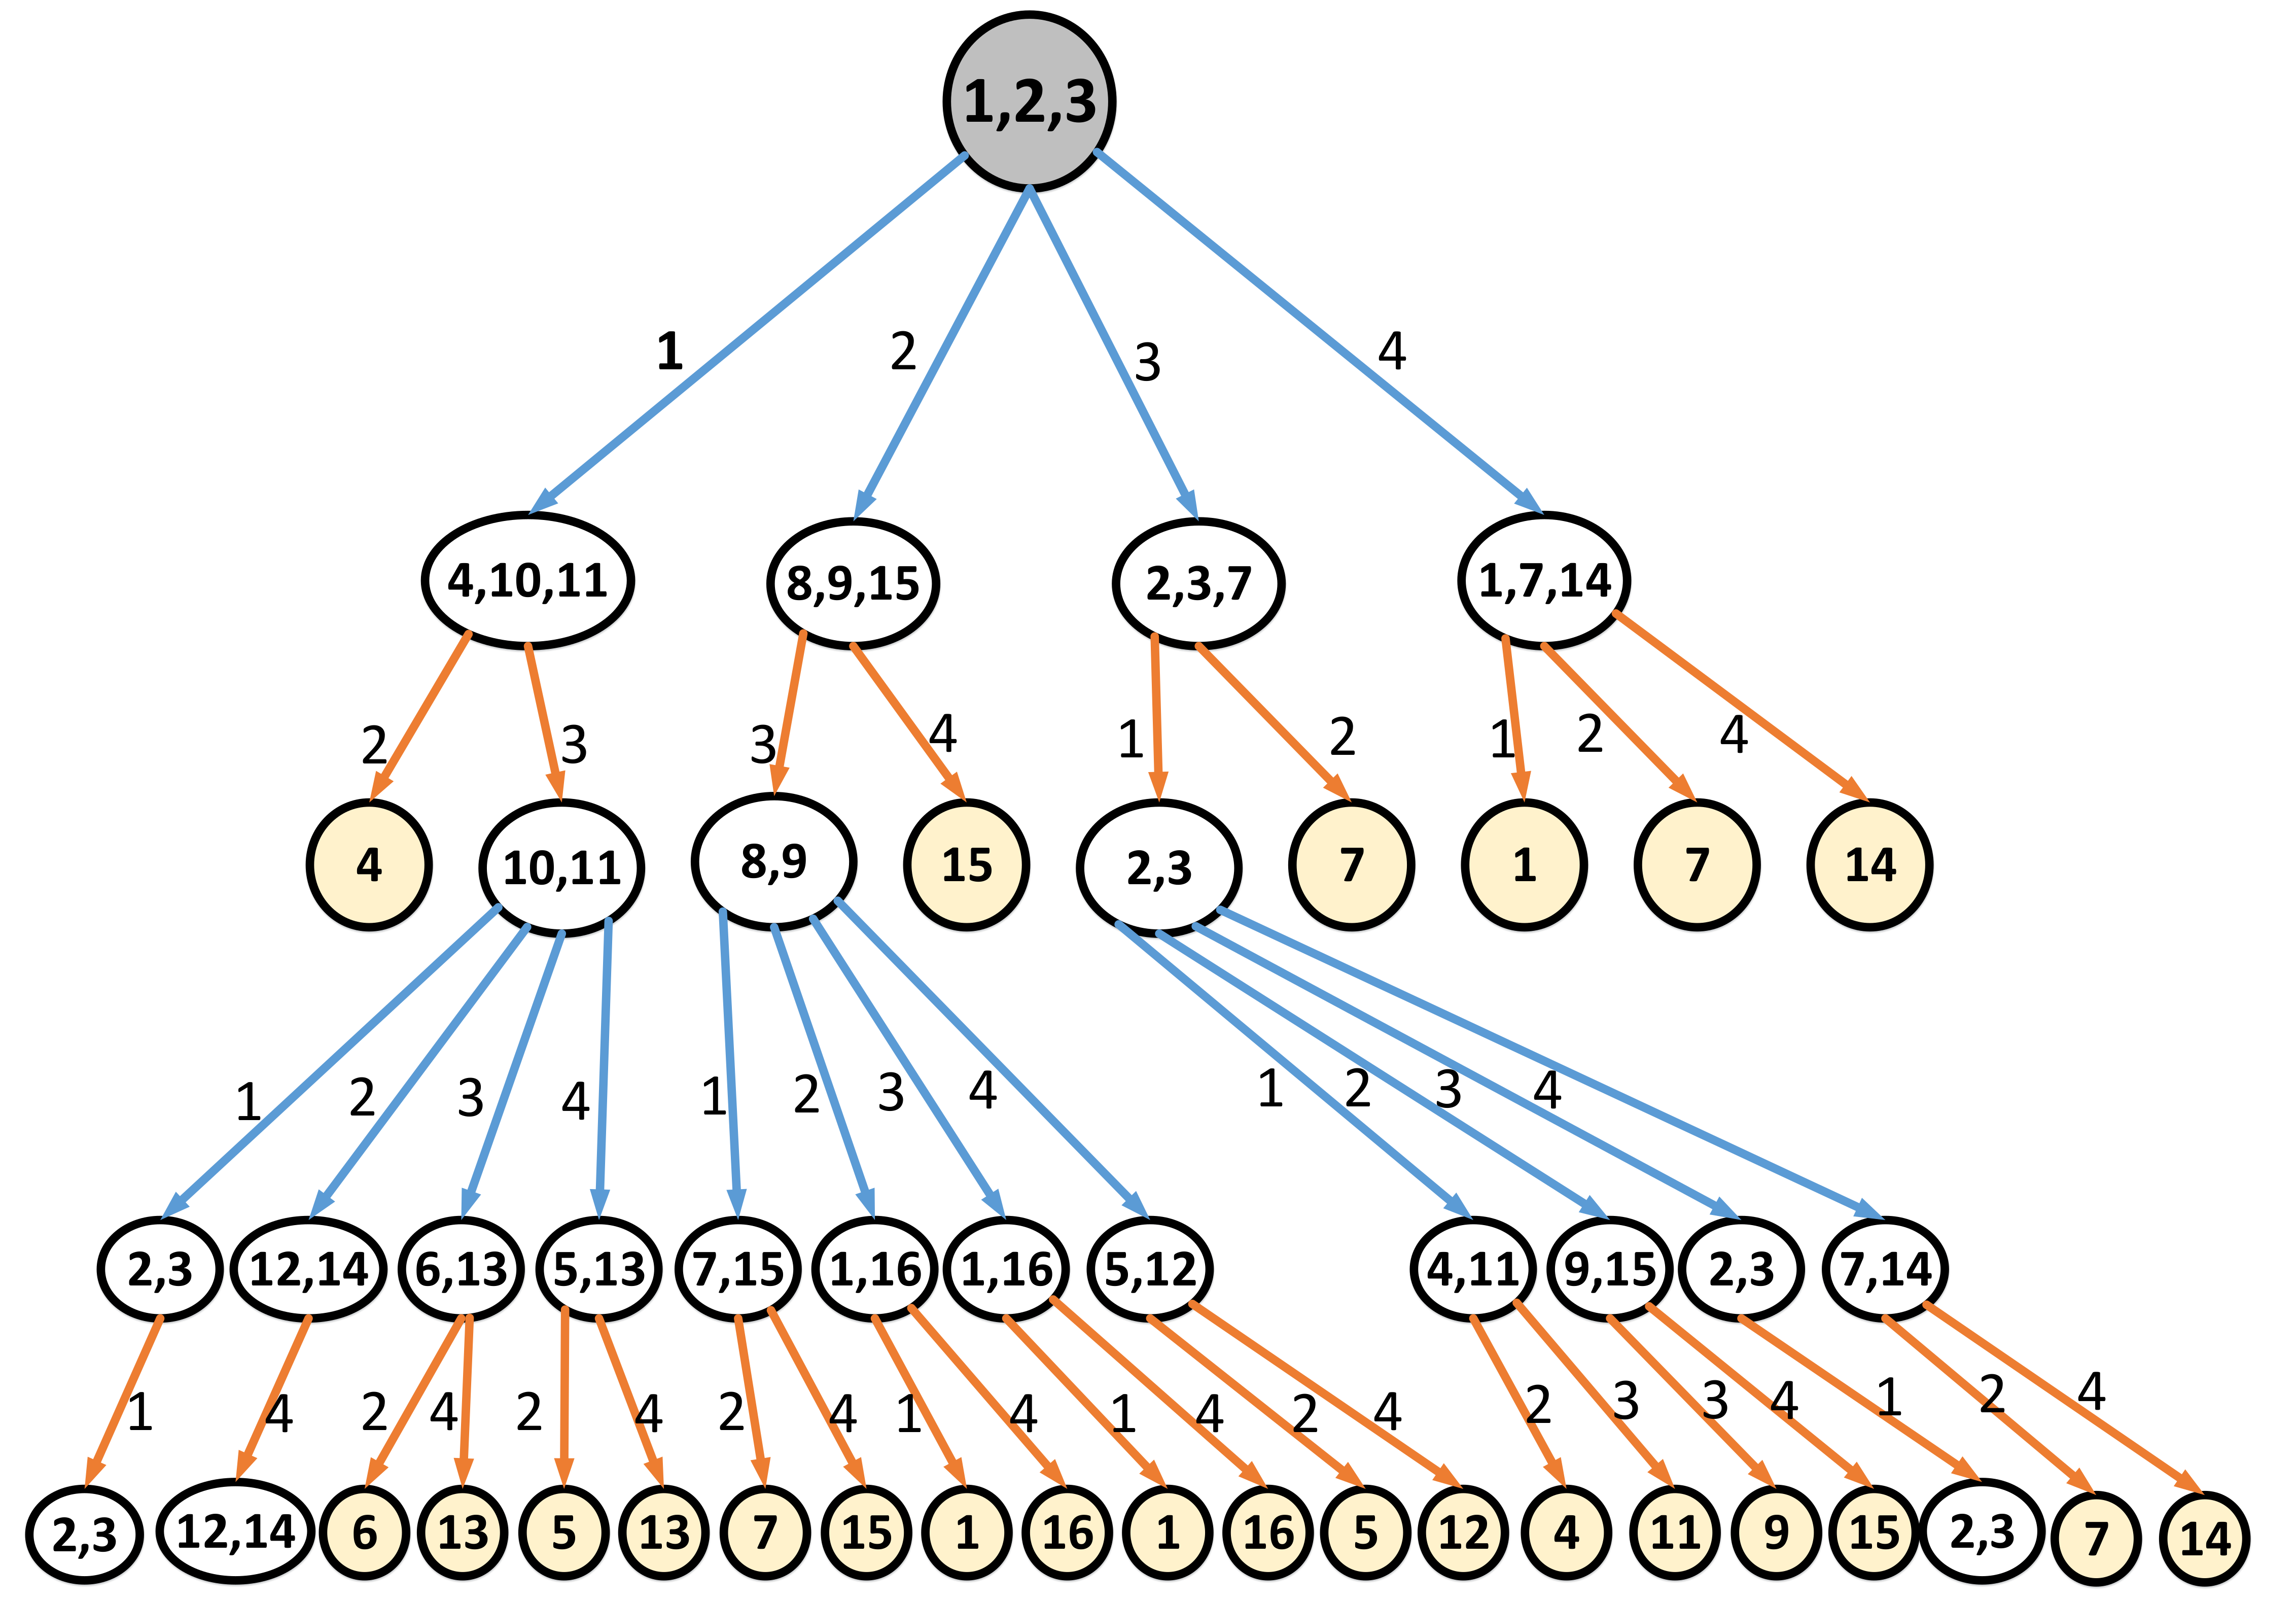
\includegraphics[scale=0.067]{figures/Fig3.png}}
	}}
      
      \caption{Branch of the super tree which represents $\{\delta_{16}^1,\delta_{16}^2,\delta_{16}^3\}$. The blue edges and orange edges show the observing output processes and deciding input processes, respectively. The yellow nodes are leaf nodes.}
      \label{fig:3}
   \end{figure}

At the beginning we infer that the possible states set is $\Delta_N$, thus the root node of the super tree is $\Delta_N$. When the cardinal number of the possible states set turns into $1$, we can determine the state of \BCN. Therefore, the leaf nodes of the super tree are the nodes with cadinal number $1$. We observe the output of \BCN\ to infer the possible states set of \BCN\ at first. After that, we decide the input and infer the new possible states set. We alternately observe the output and decide the input untill we can determine the state of {\em BCN}. Therefore we use $\Ded\left(S_i,\varepsilon, o_j\right)$ to find son nodes for every $S_i$ in $2k+1$ layer, and using $\Ded\left(S_i,i_p,\varepsilon\right)$ to find son nodes for every $S_i$ in $2k+2$ layer. The formula $|\Ded\left(S_i,\varepsilon, o_j\right)|>0$ ensures the node $\Ded\left(S_i,\varepsilon, o_j\right)$ has meaning. The formula $|\Ded\left(S_i,i_p,\varepsilon\right)|=|S_i|$ guarantee we can determine the state of \BCN\ in the end. 
\begin{example}
For example, the \BCN\ whose structure is depicted in Fig.\ref{fig:1}, and the updating rules of this \BCN\ is described as truth table in Fig.\ref{fig:2}. The Fig.\ref{fig:3} show branch of the tree which represents $\{\delta_{16}^1,\delta_{16}^2,\delta_{16}^3\}$ and its deduction process. The nodes represent the states sets, the blue edges represent the observing output processes, and the orange edges represent the deciding input processes. This branch is not completed, because only the yellow nodes are the leaf nodes. If we want to find all of the ways to determine the initial state of \BCN, we have to build the complete tree for \BCN. This process takes many additional time and space overhead. Especially when there are loops in the tree, like the $\{\delta_{16}^2,\delta_{16}^3\}$ in fourth layer and the $\{\delta_{16}^2,\delta_{16}^3\}$ in fifth layer that will form a loop. In this case we can never build the complete tree, thus we need to check the existence of loops and omit it. There are also some nodes take the same states set which will also take additional overhead. For instance there are two nodes take the same states set $\{\delta_{16}^1,\delta_{16}^{16}\}$ in the fifth layer. However, it would be a lot easier if we only need to find a way to determine the initial state. For instance, when we find the leaf nodes $\delta_{16}^1$, $\delta_{16}^7$ and  $\delta_{16}^{14}$ in third layer by breadth-first algorithm, we can make sure that the states set $\{\delta_{16}^1,\delta_{16}^2,\delta_{16}^3\}$ is 1 step deterministic. After that, we use this conclusion to determine the initial state of \BCN. 
\end{example}   
\subsection{Algorithm implemented by directed graph}
To improve the shortcomings of the way by using supertree, we proposed the way by derected graph wich may takes less time and space overhead. The most difference between supertree and derected graph is that supertree is built from the root node to leaf nodes. However, the derected graph is built from smaller nodes (contain fewer states) to larger nodes (contain more states). There is not any repeated node in the derected graph because any node only appears once in the graph. And even there are some loops in the derected graph, the loops would not influence us to build the directed graph completely.

The construction algorithm of derected graph is shown in the Algorithm.\ref{alg:1}. The algorithm to build nodes used in the Algorithm.\ref{alg:1} is shown in the Algorithm.\ref{alg:2}.

\begin{algorithm}[h]
\caption{Algorithm to construct the directed graph of \BCNs}
\begin{algorithmic}[1]
\REQUIRE 
The algebraic forms of \BCN
\ENSURE  
The directed graph of \BCN
\STATE  $k=1$ (The number of states in the nodes)\
\STATE  $Ob=$ false (The online observability of \BCN)\
\STATE  $N_i$ (Node)\
\STATE  $i_p$ (Input)\
\STATE  $NodesArray$ (Nodes array)\
\STATE  $Sis$ (The suitable inputs set of $N_i$)\
\STATE {\sf buildnode}(k)
\STATE $k= k+1$
\WHILE {NodesArray={\sf buildnode}(k)!=Null}
\STATE NodesArray={\sf buildnode}(k)
\FOR{each $N_i\in NodesArray$}
\IF{$k==2$}
\STATE $Sis$ = $\Delta_M$ 
\ELSE

\STATE Find $Sis$ by other nodes

\ENDIF
\FOR{each $i_p \in Sis$}
\STATE Check $N_i$ by $i_p$
\STATE Build edges for $N_i$ 
\ENDFOR
\IF {$N_i$ has not any edge.}
\STATE $Ob=0$ 
\STATE return Null
\ENDIF
\ENDFOR

\STATE $k= k+1$
\ENDWHILE
\STATE $Ob=1$ 
%\STATE return $Ob$
\STATE return $NodesArray$
\end{algorithmic}
 \label{alg:1}
\end{algorithm}
 The algorithm to build nodes used in the Algorithm.\ref{alg:1} is shown in the Algorithm.\ref{alg:2}.
\begin{algorithm}[h!]
\caption{{\sf buildnode}(int k)}
\begin{algorithmic}[1]
\REQUIRE 
The number of states in the nodes $k$
\ENSURE  
The nodes with $k$ states whose corresponding outputs are the same%, and the outputs of $p$ states inside one node are the same.
%\STATE {\sf buildnode}(int p)
%\STATE  \{ 
%\dfSTATE $p=p+1$\
\STATE  Build all nodes with $p$ states %(whose outputs are the same)\

\IF{Failed to build} 
\STATE  return Null
\ELSE 
\STATE  Classify these nodes
\STATE Sort the states in these nodes
\STATE Sort these nodes%(For example, the nodes $\{\delta_{16}^1,\delta_{16}^2\}$, $\{\delta_{16}^1,\delta_{16}^3\}$ and $\{\delta_{16}^2,\delta_{16}^3\}$ shown in {\em Fig.\ref{fig:4}}. )
\STATE return nodes
\ENDIF 
%\STATE \}
\end{algorithmic}
 \label{alg:2}
\end{algorithm}

Some details in Algorithm.\ref{alg:1} and Algorithm.\ref{alg:2} are as follows:
\begin{itemize}
\item Build all nodes with $k$ states: Firstly, we classify all states by their corresponding outputs, then we have all of states sets. The states set contains all states have the same corresponding outputs. Secondly, we compare $k$ with the cardinal number $Car$ of each states set $S_i$ we built before. If $k$ greater than $Car$, then we could not get $k$ states from this states set $S_i$. Else we can get $C_{Car}^k$ sets with $k$ states from this states set. Finally, we use all of states sets to build nodes we need. 
 \item Sort the states in these nodes and sort these nodes: For example, the nodes $\{\delta_{16}^1,\delta_{16}^2\}$, $\{\delta_{16}^1,\delta_{16}^3\}$ and $\{\delta_{16}^2,\delta_{16}^3\}$ shown in Fig.\ref{fig:4}. 
  \item Find $Sis$ by other nodes: The node $N_i$ with $k$ sorted states inside it, then we can use the first $k-1$ states, the last $k-1$ states and the first and last two states to find the nodes we need. And then use these three nodes to find $Sis$ for $N_i$. For example, we can search right inputs sets which make $\{\delta_{16}^4,\delta_{16}^5,\delta_{16}^6\}$, $\{\delta_{16}^5,\delta_{16}^6,\delta_{16}^7\}$ and $\{\delta_{16}^4,\delta_{16}^7\}$ $k$-step deterministic at first. After that, take the intersection of these sets to be the suitable inputs set of $\{\delta_{16}^4,\delta_{16}^5,\delta_{16}^6,\delta_{16}^7\}$. 
  \item Check $N_i$ (with states set $S_i$ in it) by $i_p$: According to the order determined in previous steps, we check every node in order. If for one input $i_p$ (which belongs to suitable inputs set $Sis$) implies $|\Ded\left(S_i,i_p,\varepsilon\right)|<|S_i|$, we can make sure the $i_p$ is a wrong input. Else if for each $O_j \in \Delta_Q$, $|\Ded\left(S_i,i_p,o_j\right)|>0$ and $\Ded\left(S_i,i_p,o_j\right)$ is $k$-step deterministic then $I_j$ is a right input. Therefore, we can connect the node $S_i$ to each node $\Ded\left(S_i,i_p,o_j\right)$ with directed edge. The colour of directed edges represent its corresponding input. Else if there exist $o_j \in \Delta_Q$ and we can not make sure whether $\Ded\left(S_i,i_p,o_j\right)$ is $k$-step deterministic, we check it in the next round. 
\end{itemize} 

According the construction process, we have the definition of directed graph.
\begin{definition}[Directed Graph]
Every node $S_i$ in the directed graph is $k$-step deterministic, and there are no duplicate nodes in the graph. For every distinct two $s_a, s_b \in S_i$ we have $Hs_a=Hs_b$. If $|S_i|=1$, then there are not edge from it to other nodes, else if there are exist one edge $i_p$ from it to one nodes then there exist $z$ ($z\ge 1)$ edges contain $i_p$ from it to nodes $S_1,\ldots,S_z$ that \[|S_i|= |S_1|+,\ldots,|S_z|\] and \[\Ded\left(S_i,i_p,\varepsilon\right)=S_1\vee,\ldots,\vee S_z.\]
\end{definition}

When we trying to build the directed graph for a \BCN, we check whether the nodes with fewer states are $k$-step deterministic first and then check whether the nodes with more states are $k$-step deterministic.  As the the nodes with fewer states are not $k$-step deterministic, the nodes with more states would not be $k$-step deterministic. Therefore, once we can find a node is not $k$-step deterministic we can know that $\Delta_N$ is not $k$-step deterministic and this \BCN\ is not online observable. Moreover, we can use the nodes with fewer states that are $k$-step deterministic to help us check the nodes with more states. For instance, if the node $S$ has two edges from it to two nodes $S_1$ and $S_2$, and we have $S_1$ and $S_2$ are $k$-step deterministic. In this case, we can make sure that the node $S$ is $k$-step deterministic.

Based on the definitions of existing four kinds of observability, we can also use the directed graph to determine the existing second and fourth kinds of observability. When we trying to build bottom layer and penultimate layer of the directed graph, if there are exist some nodes in penultimate layer has no edges from it to other nodes. In this case this \BCN\ is not satisfied existing second observability. When we trying to build edges for every layer, and if there exist one node whose right inputs set is not $\Delta_M$, then this BCN is not satisfied existing fourth observability.
\begin{figure}[thpb]
      \centering
      \framebox{\parbox{3in}{
		\centerline{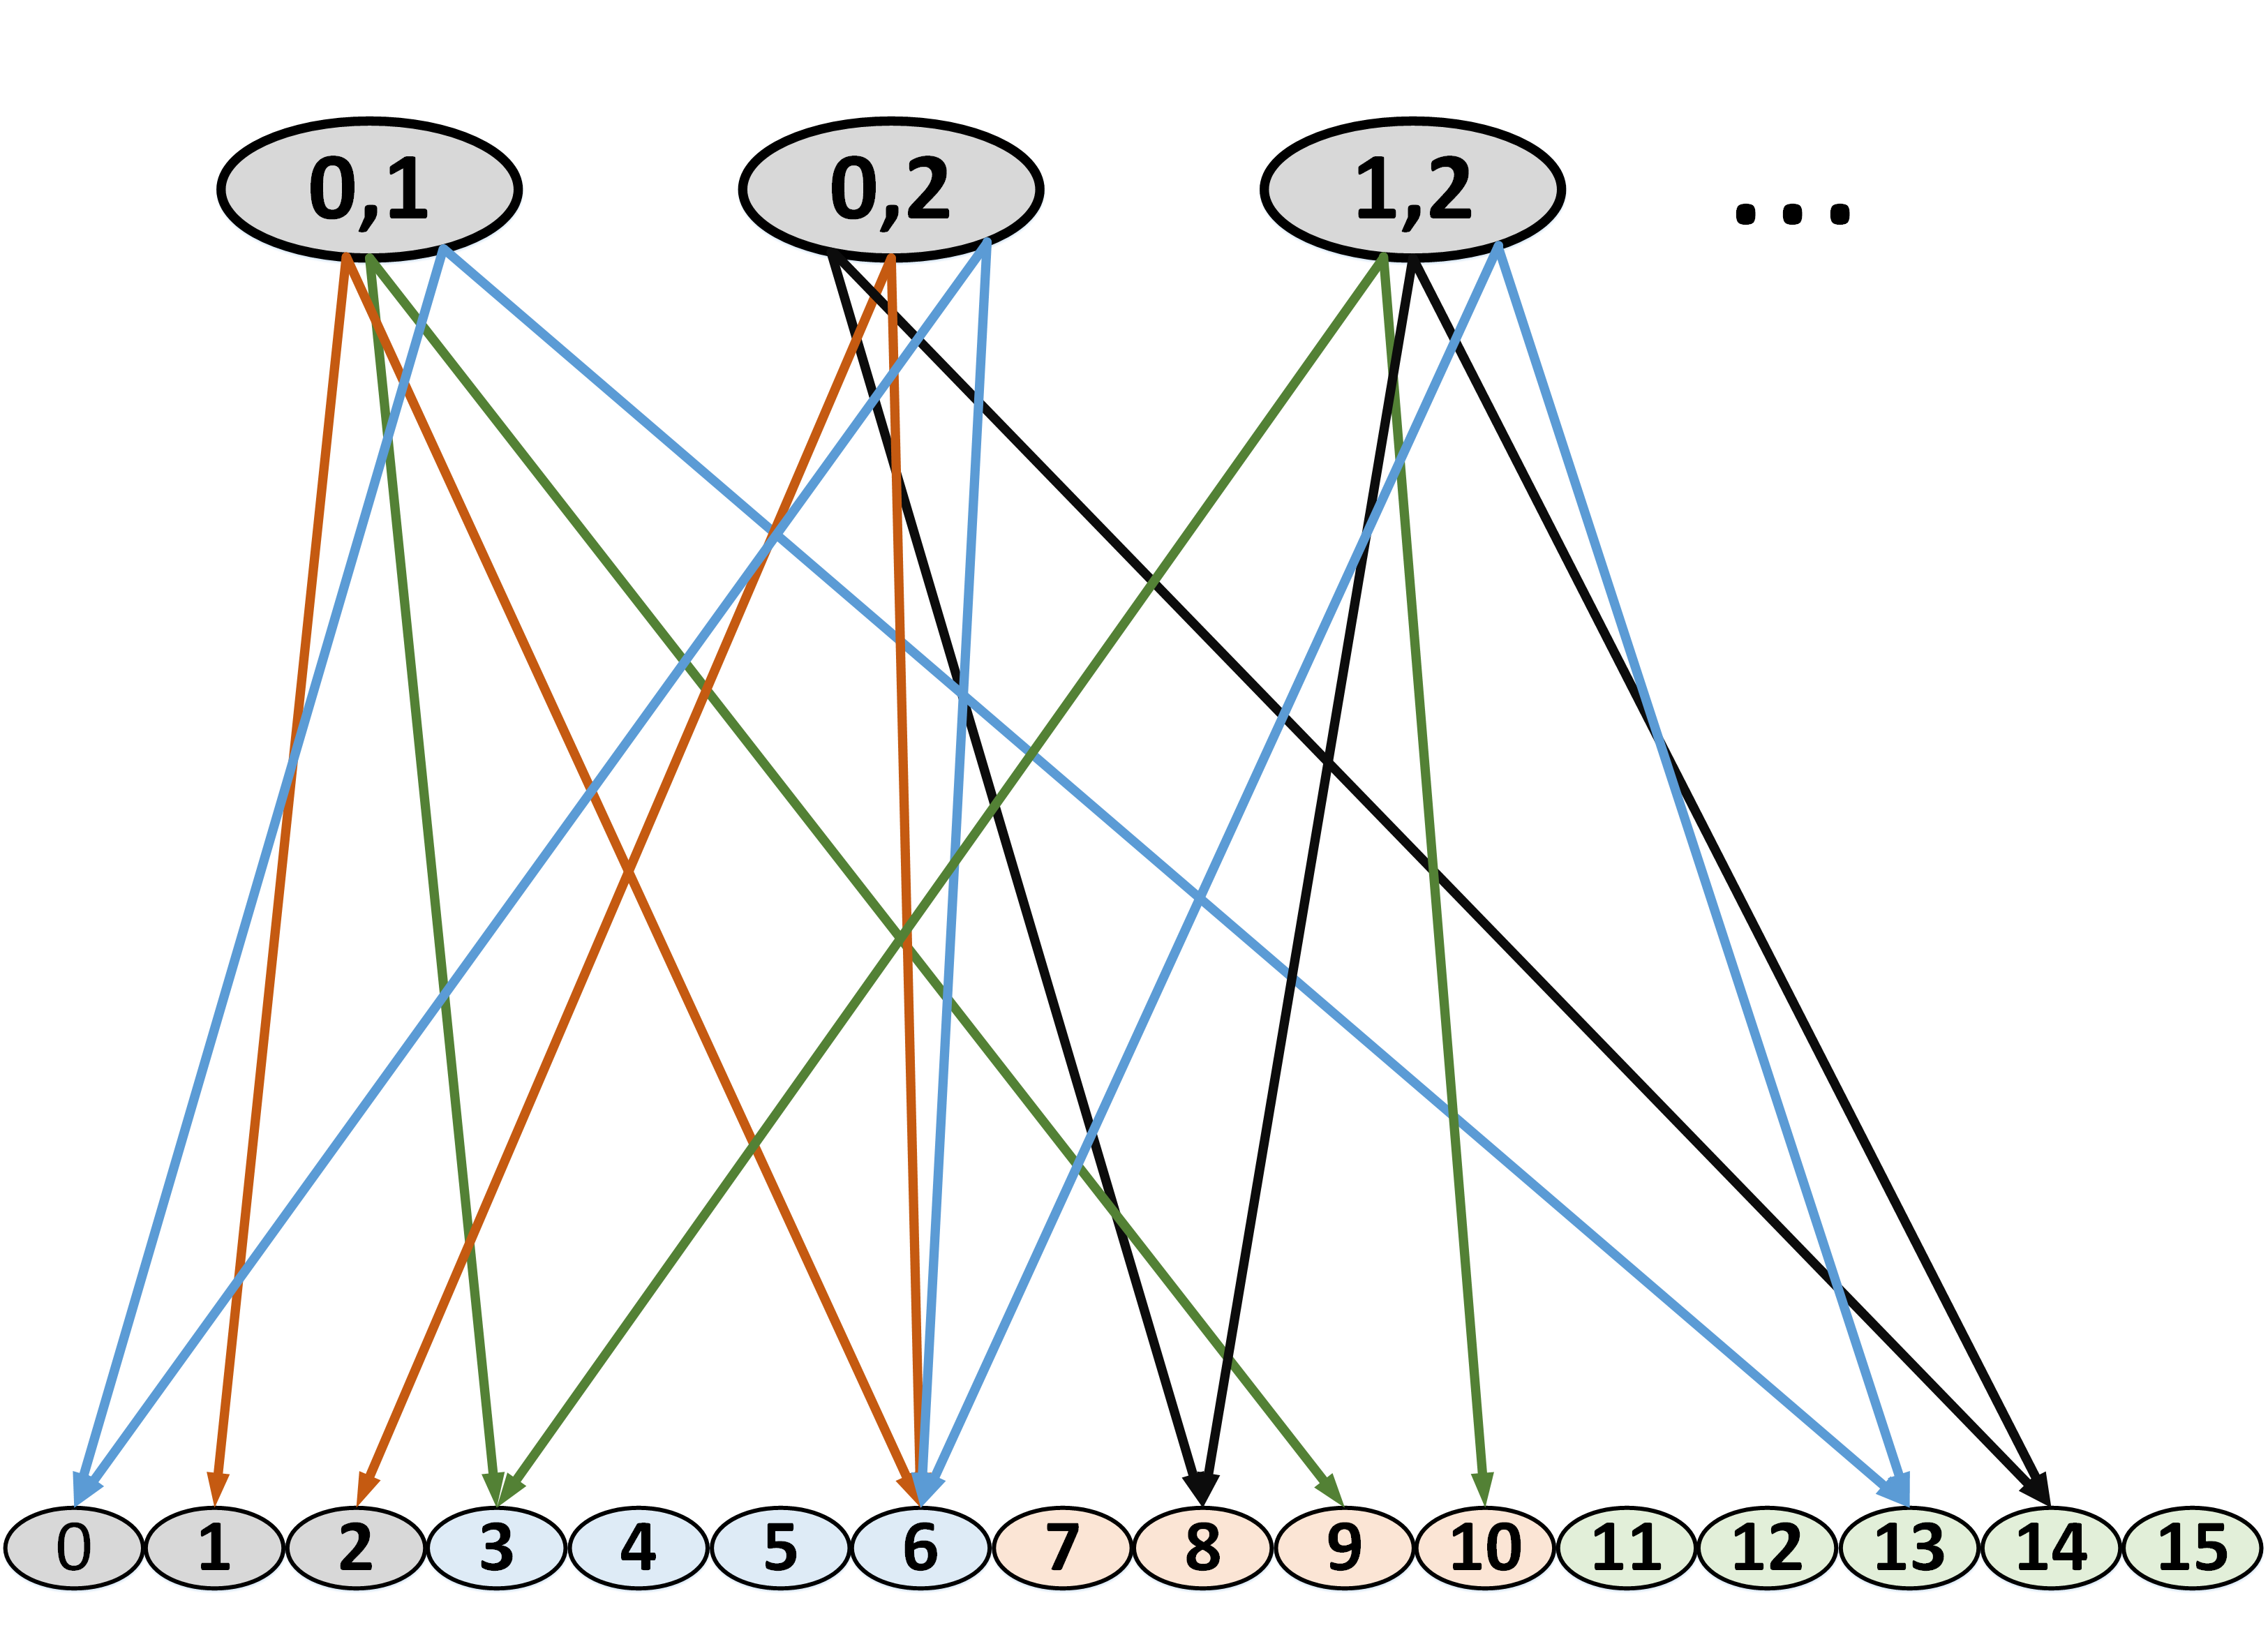
\includegraphics[scale=0.090]{figures/Fig4.png}}
	}}
      
      \caption{Part of the directed graph which represents $\{\delta_{16}^1,\delta_{16}^2\}$, $\{\delta_{16}^1,\delta_{16}^3\}$ and $\{\delta_{16}^2,\delta_{16}^3\}$. The green, black, orange, blue edges show the inputs $\delta_4^1$, $\delta_4^2$, $\delta_4^3$ and $\delta_4^4$ respectively.}
      \label{fig:4}
   \end{figure}
\subsection{Complexity analysis}
The way by the directed graph is better than by supertree, thus we analyze the complexity of it. We classify the states with their corresponding output. After that form the set of states set $\{S_1, S_2,\ldots,S_M\}$,  and every element in a states set has the same corresponding output. That is to say, for each $S_i\in\{S_1, S_2,\ldots,S_M\}$ then for every $s_k\in S_i$ we have $Hs_k=\delta_{M}^i$.

Firstly, we need to calculate the upper bound of the number of the states in the directed graph nodes $k$ we have.
\begin{equation}
\begin{split}
k_{upb}= \max(|S_1|,|S_2|,\ldots,|S_M|)
\end{split}
\end{equation}
The $ k_{upb}$ is the maximum value of $|S_1|,|S_2|,\ldots,|S_M|$, because the states in the directed graph nodes should have the same corresponding output.

Secondly, we need to calculate the number of nodes with $k$ states:
\begin{equation}
\begin{split}
k_{non}= C_{|S_i|}^k+\ldots +C_{|S_p|}^k
\end{split}
\end{equation}
where $S_i\ldots,S_p\in\{S_1, S_2,\ldots,S_M\}$ and $|S_i|,\ldots,|S_p|\ge k$.

Thirdly we need to calculate the cardinal number of suitable inputs set of each node. Finally we need to calculate the time used to check each input is a right input for a node.

After completing the previous steps, calculate the complexity by layer by layer. But the cardinal number of suitable inputs set of a node depends on the cardinal number of it and the other three nodes used to find the suitable inputs set for it. And the time used to check whether an input is a right input for a node also depends on the updating rules of {\em BCNs}.

Moreover, instead of taking $\Delta_M$ as the suitable inputs set for every node in thedirected graph. We would use the other three nodes like $\{\delta_{16}^4,\delta_{16}^5,\delta_{16}^6\}$, $\{\delta_{16}^5,\delta_{16}^6,\delta_{16}^7\}$ and $\{\delta_{16}^4,\delta_{16}^7\}$ that are $k$-step deterministic to find the suitable inputs set for a node $\{\delta_{16}^4,\delta_{16}^5,\delta_{16}^6,\delta_{16}^7\}$ with more than $2$ states. By this way we can  reduce the cardinal number of the suitable inputs set for every nodes with more than 2 states, and then reduce the time cost. 

The reason why we can use this method is that only the input which make the subset of $\{\delta_{16}^4,\delta_{16}^5,\delta_{16}^6,\delta_{16}^7\}$ $k$-step deterministic will make the $\{\delta_{16}^4,\delta_{16}^5,\delta_{16}^6,\delta_{16}^7\}$ $k$-step deterministic. Furthermore, using these three nodes will be a good way to cover all the subset with cardinal number $2$ of $\{\delta_{16}^4,\delta_{16}^5,\delta_{16}^6,\delta_{16}^7\}$. That is to say every subset $s_i$ with cardinal number $2$ included in $\{\delta_{16}^4,\delta_{16}^5,\delta_{16}^6,\delta_{16}^7\}$ will included in $\{\delta_{16}^4,\delta_{16}^5,\delta_{16}^6\}$, $\{\delta_{16}^5,\delta_{16}^6,\delta_{16}^7\}$ or $\{\delta_{16}^4,\delta_{16}^7\}$. This conclusion can help us to select the nodes we need when we seek the suitable inputs set for a node. But it is hard to analyze the complexity of this method, and it makes the complexity analysis of the way by directed graph harder.

Therefore, it is hard to give a accurate complexity of the algorithm without the complete imformation of \BCNs. We may finish this job in the furture, and we will try to use real example to do complexity analysis.
%Because the states in a nodes will have the same corresponding output, so we have the upper bound of the number of the states in a directed graph nodes $k$: We classify the states with their corresponding output and form the set of states with the same corresponding output, the greatest cardinal number of these set would be the upper bound of $k$. 
%% !Mode\dots ``TeX:UTF-8''
% !TEX root = ../root.tex
\section{Applications}
\label{sec:app}
If we research the systems described by \BCNs\ which are online observable but not satisfy the existing third and fourth observability, we can only use the online observability to determine their initial state in real time. If we have built the corresponding directed graphs for them, we can use the online observability to determine the initial state of these \BCNs. In addition, online observibility requires less observation costs for us to determine the initial state of some systems described by  \BCNs\ in real time. Furthermore we can also use the online observability to find the shortest path or avoid entering critical states in the process of determining the initial state of \BCNs. %Because the output we observe is not sure, we use expected value and variance of the length of path and the times of entering critical states to help us to choose the input.

\subsection{Determining initial state}

If a system described by \BCN\ is online observable but not satisfy the existing third and fourth observability. And the directed graph of a it has been built, then we can determine the initial state of this system (or \BCN) in real time by online observability. To illustrate the process of determining the initial state of a \BCN, we give one example is as follows.
\begin{example}
The \BCN\ whose structure is depicted in Fig.\ref{fig:1}, and the updating rules of this \BCN\ is described as truth table in Fig.\ref{fig:2}. The process of determining its initial state is as {\em Fig.\ref{fig:5}} shows. 
\begin{itemize}
  \item Firstly, we observe the output of the \BCN\ mentioned before. If we observe the output is $\delta_4^1$ then we can infer that the possible states set should be $\{\delta_{16}^1,\delta_{16}^2,\delta_{16}^3\}$, and we record them as initial states and current states in the table. 
  \item After that we input  $\delta_4^1$ and observe the output is $\delta_4^3$ then we can infer that the possible states set should be $\{\delta_{16}^{10},\delta_{16}^{11}\}$, and we record them as current states set in the corresponding position. 
 \item Repeat the second step untill the cardinal number of the possible states set turns into $1$. In that time we can determine the current state ($\delta_{16}^{6}$) and the corresponding initial state  ($\delta_{16}^{3}$) of the {\em BCN}.
\end{itemize} 
\end{example}   
%Input and output again and again 

\begin{figure}[thpb]
      \centering
      \framebox{\parbox{3in}{
		\centerline{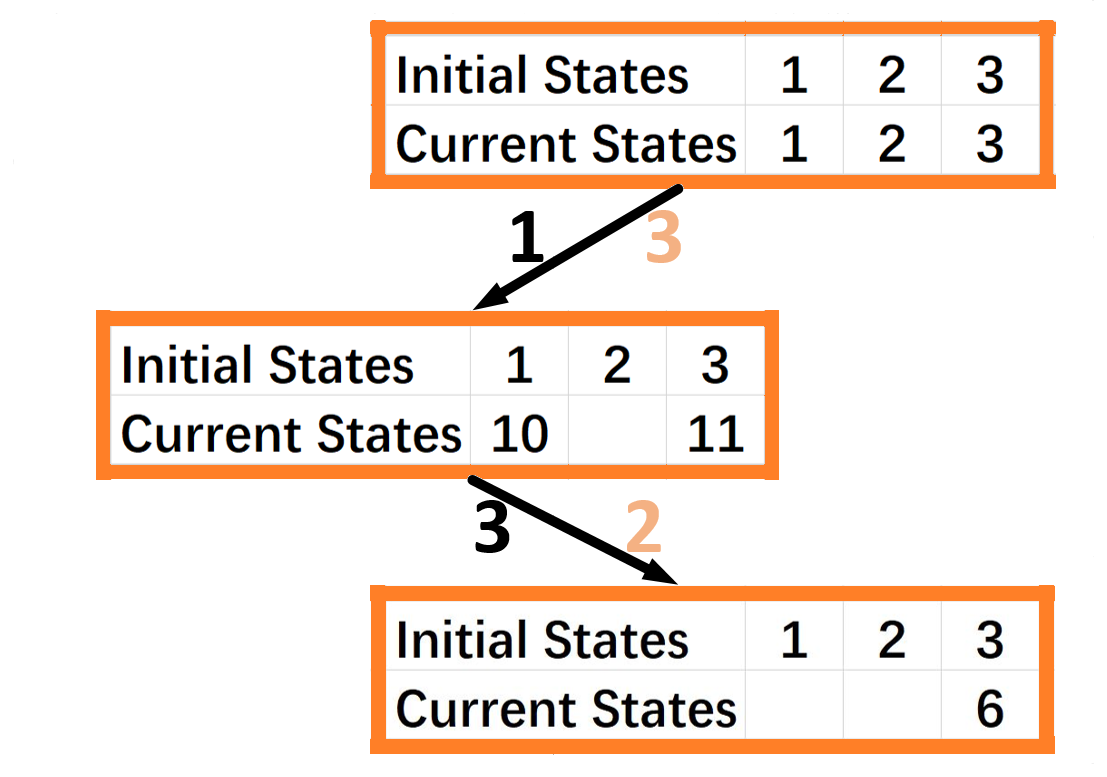
\includegraphics[scale=0.266]{figures/Fig5.png}}
	}}
      
      \caption{The process of determing the initial state of BCNs, we change the values of current states by input and the output we observe. }
      \label{fig:5}
   \end{figure}
%\subsection{Less observation costs}
In addition, it takes less observation costs for us to determine the initial state of some systems described by \BCNs. There are some biological systems depicted by \BCNs, such as the immune systems which can be depicted as the \BCN\ T-cell receptor kinetics model \cite{Klamt2006A}. And there exist $3$ input-nodes, and $37$ state-nodes in this model, therefore the model has $2^3$ inputs and $2^{37}$ states. For the purpose of obtain the initial state of this \BCN, we must select some state-nodes to be observe at first, and it would take many costs for us to observe the state-node values. However, if we use the online observability of \BCNs\ to determine the initial state of the \BCN\ T-cell receptor kinetics model in real time. It needs less observation costs than the existing third and fourth observability. Because compared with the existing third and fourth kind of observability the online observability needs weakest preconditions to determine the initial state of \BCNs\ in real time. In other words, we need fewer output-nodes (or state nodes to be observed) of the \BCN\ T-cell receptor kinetics model to determine its initial state. We need fewer state-nodes to be observe, then it will takes less ovservation costs in this \BCN\ T-cell receptor kinetics model. In addition, there are also some other advantages of the online observability of \BCNs.

\subsection{Finding shortest path}
When we need to determine the initial state of a \BCN, an important aspect that we will consider is to find the shortest path to determine the initial state. In general, we can not find the shortest path definitely.  Fortunately, we can use the directed graph to make the best decision. For the path, we introduce two functions $\Pe(S, i_p)$ and $\Pv(S, i_p)$ to describe its expected value and variance, respectively. In order to better explain our idea, we define some functions in the following.

%We introduce two functions $Spe(S_i, I_i)$ and $Spv(S_i, I_i)$ to describe the expected value of the shortest path and variance of shortest path , $S_i$ is the possible states set and $I_i$ is the input we chose, the definition of $Spe(S_i, I_i)$ is as follows:\\
%With the $Spe(S_i, I_i)$ and $Spv(S_i, I_i)$ we can make the decision we like.


Some necessary statements before defining the functions $\Pe(S, i_p)$ and $\Pv(S, i_p)$:
\begin{itemize}
  \item $S$: the set of states.
  \item $\{i_1,i_2,\ldots, i_z\}$ : the right inputs set of $S$;
  \item $\{S_p^1,S_p^2,\ldots, S_p^k\}$ : the set of state sets, and its elements corresponding to the possible outputs $\{o_1,o_2,\ldots,o_k\}$. As we choose the input $i_p$ to determine initial state by $S$, for each $i_p$ in $\{i_1,i_2,\ldots, i_z\}$.
 % \item the fourth one implies the third one, second one and first one.
\end{itemize} 
\begin{definition}[$\Spe(S)$] \label{lspe}
 \[\Spe(S)= \min(\Pe(S, i_1),\Pe(S, i_2),\ldots,\Pe(S, i_z)).\] 
\end{definition}

\begin{definition}[$\Pe(S, i_p)$] 
When the $|S|=1$, we have that
$\Pe(S, i_p)=0$  for every $i_p$ in $\{i_1,i_2,\ldots, i_z\}$. According {\em Definition \ref{lspe}}, $\Spe(S)=0$ if $|S|=1$. But when the $|S|>1$, 
%and the $\{I_1,I_2,\cdots, I_p\}$ is the right inputs set of $S_i$. For every $I_i$ in $\{I_1,I_2,\cdots, I_p\}$ the $\{S_i^1,S_i^2,\cdots, S_i^k\}$ is a set of state sets whose elements corresponding to the possible outputs after input $I_i$, then 
we have that  
\[\Pe(S, i_p)=1 +\frac{\sum_{j=1}^k \Spe(S_p^j)|S_p^j|}{ |S|}\] 
%and 
%\[{\tt Spe}(S_i)= \min({\tt Pe}(S_i, I_1),{\tt Pe}(S_i, I_2),\cdots,{\tt Pe}(S_i, I_p))\]
\end{definition}

The function shortest path  expected value $\Spe(S)$ is to find the $i_p$ from $\{i_1,i_2,\ldots, i_z\}$ to calculat least $\Pe(S, i_p)$ for $S$. From the definition of $\Pe(S, i_p)$ we can know that if $|S|=1$ then we can make sure the state of \BCNs, that we need not choose the input anymore to determine the state of \BCNs. Therefore, for any input the path expected value $\Pe(S, i_p)$ would be $0$ and the shortest path expected value $\Spe(S)$ also would be $0$. But if $|S|>1$ we still need to choose input and observe the output. Only by this way we can determine the state of of \BCNs. Therefore, we can recursively define the $\Pe(S, i_p)$ and $\Spe(S)$ for each input $i_p$ in the right inputs set. The $\Pv(S, i_p)$ is defined in the similar way. Hence we omit the details of the definition of $\Pv(S, i_p)$ in this paper. \\

If we want to find the shortest path to determine the initial state of a \BCN, we can choose an input $i_p$ with least $\Pe(S, i_p)$. This input $i_p$ may help us find the shortes path to determine the initial state. But the output of \BCNs\ is uncertain after we choose the input $i_p$, hence selecting the $i_p$ which with least $\Pe(S, i_p)$ may leads to a very long path to determine the initial state of \BCNs. For better performce, we the can use the $\Pv(S, i_p)$ to avoid this risk. If the $\Pv(S, i_p)$ of input $i_p$ with is not very large, the risk after choosing $i_p$ would be not great too.
\subsection{Avoiding entering critical states}
In biological systems, some states of the genes may corresponding to unfavorable or dangerous situations \cite{Li2014Controllability}. So another important aspect that we consider is to avoid entering critical states in the process of determining the \BCN's initial state. Therefore, we construct two functions $\Ce(S, i_p)$ and $\Cv(S, i_p)$ to describe expected value and variance of the times of entering critical states too, the definition of $\Ce(S, i_p)$ is as follows.\\
\begin{definition}[$\Lce(S)$] \label{lce}
\[\Lce(S)= \min(\Ce(S, i_1),\Ce(S, i_2),\ldots,)\Ce(S, i_z)\]
\end{definition}
\begin{definition}[$\Ce(S, i_p)$] 
When the $|S|=1$, and for every $i_p$ in $\Delta_M$, we have: \[\Ce(S, i_p)=|S \cap S_{cri} |\] 
According {\em Definition \ref{lce}}, %{\tt Spe}$(S_i)=0$ if $|S_i|=1$ 
\[\Lce(S)=\Ce(S, i_p)=|S \cap S_{cri} |\] 
But when the $|S|>1$ 
%and the $\{I_1,I_2,\cdots, I_p\}$ is the right inputs set of $S_i$. For every $ I_i$ in $\{I_1,I_2,\cdots, I_p\}$ the $\{S_i^1,S_i^2,\cdots, S_i^k\}$ is a set of state sets whose elements corresponding to the possible outputs after input $I_i$, then 
we have that 
\[\Ce(S, i_p)=|S \cap S_{cri} | +\frac{\sum_{j=1}^k \Lce(S_p^j)|S_p^j|}{ |S|} \] 
%and 
%\[{\tt Lce}(S_i)= \min({\tt Ce}(S_i, I_1),{\tt Ce}(S_i, I_2),\cdots,){\tt Ce}(S_i, I_p)\]
\end{definition}

Where $S_{cri}$ is the critical states set of the \BCN\ we research. The definition of $\Ce(S, i_p)$ has some difference with $\Pe(S, i_p)$, because we need to use the critical states set $S_{cri}$. So that  we can analyze the possibility of entering the  critical states when we infer the possible states set of \BCNs, and we can get the definitions of $\Cv(S, i_p)$ in similar ways. We omit the details of the definition of $\Cv(S, i_p)$ in this paper as well. 

The use of $\Ce(S, i_p)$ and $\Cv(S, i_p)$ are similar to $\Pe(S, i_p)$ and $\Pv(S, i_p)$ respectively. They help us avoid entering critical states of \BCNs\ in the process of determining the initial state of \BCNs. With these four functions $\Ce(S, i_p)$, $\Cv(S, i_p)$, $\Ce(S, i_p)$ and $\Cv(S, i_p)$, we can make the best decision we like. 

In the four existing kinds of observability, they have not property {\em interactivity}. We can not analyze the state of \BCNs\ dynamically, hence it would be hard to find the best path we like in the process of determining the initial state of \BCNs. However, this problem can be solved by the online observability of \BCNs\ better.
% !Mode\dots ``TeX:UTF-8''
% !TEX root = ../root.tex
\section{Conclusions}
\label{sec:con}
In this paper, firstly we proposed the online observability of {\em BCNs} and define its mathematical form. Secondly we use the super tree and directed graph to determine the online observability. After introduced the ways to determine the online observability we present some applications of the online observability of {\em BCNs} and talk about some advantages of it. 
%use it to try to find the shortest path and avoid entering critical states when we determining the initial state of {\em BCNs}. 

But even we use the directed graph, it is still hard to determine the  the online observability of a \BCN\ with a large number of nodes. Therefore, in the future we will try to separate the {\em BCNs}, and then determine their online observability respectively. Furthermore, we also want to try to use some knowledge about formal methods to earn scalability for {\em BCNs}. In addition to the theoretical aspect, the realistic application is also very important. Hence we will also try to find some realistic example which can be modeled by {\em BCNs}. So that we can research these realistic examples well and determine the online observability their models for better performance.
\bibliographystyle{IEEEtran} 
\bibliography{bcn} 
\begin{appendices}
\section{Proof}
\label{sec:pro}
\subsection{Proof of Lemma \ref{lemm:1}}
\begin{proof}
%$\mathsf{S}^{1}\subseteq \mathsf{S}^{2}$, 
If $\Ks(\mathsf{S}^{2})=0$, we have  \[\mathsf{S}^{1} = \mathsf{S}^{2}.\] Therefore, we have $\Ks(\mathsf{S}^{1})=0\le\Ks(\mathsf{S}^{2})$, thus we have the {\em Lemma \ref{lemm:1}} is right when $\Ks(\mathsf{S}^{2})=0$.
 
 If for $\Ks(\mathsf{S}^{2})=0,\ldots, k$ the {\em Lemma \ref{lemm:1}} is right. When $\Ks(\mathsf{S}^{2})=k+1$, we have for $\mathsf{S}^{2}$ there exists a $\mathsf{i}\in \mathcal{I}$ such that
 \begin{itemize}
 \item  $|\Ded\left(\mathsf{S}^{2},\mathsf{i},\varepsilon\right)|=|\mathsf{S}^{2}|$, and 
 \item  $\Ks(\Ded(\mathsf{S}^{2},\mathsf{i},\mathsf{o}))<(k+1)$, for each non-empty $\Ded(\mathsf{S}^{2},\mathsf{i},\mathsf{o})$.
 \end{itemize}
 and there is not any $\mathsf{i} \in \mathcal{I}$ satisfies that
  \begin{itemize}
 \item  $|\Ded\left(\mathsf{S}^{2},\mathsf{i},\varepsilon\right)|=|\mathsf{S}^2|$,
 \item  $\Ks(\Ded\left(\mathsf{S}^{2},\mathsf{i},\mathsf{o}\right))< k$ for each non-empty $\Ded\left(\mathsf{S}^{2},\mathsf{i},\mathsf{o}\right)$.
 \end{itemize} 
 Then we have for $\mathsf{S}^{1}$ there exists a $\mathsf{i}\in \mathcal{I}$ such that
 \begin{itemize}
 \item  $|\Ded\left(\mathsf{S}^{1},\mathsf{i},\varepsilon\right)|=|\mathsf{S}^{1}|$, and 
 \item  $\Ks(\Ded(\mathsf{S}^{1},\mathsf{i},\mathsf{o}))<(k'+1)\le (k+1)$, for each non-empty $\Ded(\mathsf{S}^{1},\mathsf{i},\mathsf{o})\subseteq \Ded(\mathsf{S}^{2},\mathsf{i},\mathsf{o}^{j})$.
 \end{itemize}
 and there is not any $\mathsf{i} \in \mathcal{I}$ satisfies that
  \begin{itemize}
 \item  $|\Ded\left(\mathsf{S}^{1},\mathsf{i},\varepsilon\right)|=|\mathsf{S}^1|$,
 \item  $\Ks(\Ded\left(\mathsf{S}^{1},\mathsf{i},\mathsf{o}\right))<k'\le k$ for each non-empty $\Ded\left(\mathsf{S}^{1},\mathsf{i},\mathsf{o}\right)$, $\Ded\left(\mathsf{S}^{1},\mathsf{i},\mathsf{o}\right)\subseteq \Ded\left(\mathsf{S}^{2},\mathsf{i},\mathsf{o}\right)$,
 \end{itemize} 
 Therefore we have if for $\Ks(\mathsf{S}^{2})=0,\ldots, k$ the {\em Lemma \ref{lemm:1}} is right, then when $\Ks(\mathsf{S}^{2})=k+1$ the {\em Lemma \ref{lemm:1}} is right too. 
And we have the {\em Lemma \ref{lemm:1}} is right when $\Ks(\mathsf{S}^{2})=0$. Thus we have the {\em Lemma \ref{lemm:1}} is right for every $\Ks(\mathsf{S}^{2})\ne \infty$.
 
\end{proof}
\subsection{Proof of Lemma \ref{lemm:2}}
\begin{proof}
For the non-empty $\mathsf{S}^{1}$ and $\mathsf{S}^{2}$, if $\mathsf{S}^{1}\subseteq\mathsf{S}^{2}$ and $\Ks(\mathsf{S}^{2})\ne\infty$.
For every $\mathsf{i}\in \Ri(\mathsf{S}^2)$, we have  $|\Ded\left(\mathsf{S}^2,\mathsf{i},\varepsilon\right)|=|\mathsf{S}^2|$, and 
for every $\mathsf{o} \in \mathcal{O}$, $\Ded(\mathsf{S}^2,\mathsf{i},\mathsf{o})\ne \emptyset$ implies $\Ks(\Ded(\mathsf{S}^2,\mathsf{i},\mathsf{o}))\ne \infty$. With {\em Lemma \ref{lemm:1}} we have $|\Ded\left(\mathsf{S}^1,\mathsf{i},\varepsilon\right)|=|\mathsf{S}^1|$, and 
for every $\mathsf{o} \in \mathcal{O}$, $\Ded(\mathsf{S}^1,\mathsf{i},\mathsf{o})\ne \emptyset$ implies $\Ks(\Ded(\mathsf{S}^1,\mathsf{i},\mathsf{o}))\le \Ks(\Ded(\mathsf{S}^2,\mathsf{i},\mathsf{o}))$, thus $\mathsf{i}\in \Ri(\mathsf{S}^1)$. Therefore, $\Ri(\mathsf{S}^2)\subseteq\Ri(\mathsf{S}^1)$.
\end{proof}


\subsection{Proof of Lemma \ref{lemm:3}}
\begin{proof} Firsrly, we prove the propostion that for a set of possible state $\mathsf{S}(t)$ if $\Ks(\mathsf{S}(t))\ne\infty$, then for every state \State$(t)\in \mathsf{S}(t)$, there exists an input sequence $\mathsf{I}\in(\mathcal{I})^{k}$ for some $k >0$ such that for every $\mathsf{s}'(t)\in \mathsf{S}(t)$, $\mathsf{s}'(t)\neq \mathsf{s}(t)$ implies $(HF)^{k}_{\mathsf{s}'(t)}(\mathsf{I})\neq (HF)^{k}_{{\mathsf{s}(t)}}(\mathsf{I})$.
\begin{itemize}
\item When $\Ks(\mathsf{S}(t))=0$, we have $|\mathsf{S}(t)|=1$, then for every \State$(t)$$\in \mathsf{S}(t)$ there does not exist any $\mathsf{s}'(t)\in \mathsf{S}(t)$ that $\mathsf{s}(t)\neq \mathsf{s}(t)$. Therefore, we have that for any $k >0$, for every input sequence $\mathsf{I}\in(\mathcal{I})^{k}$ the propostion is right. 
\item If for $\Ks(\mathsf{S}(t))=0,\ldots, n$ the propostion is right. When $\Ks(\mathsf{S}(t))=n+1$, we have for $\mathsf{S}(t)$ there exists a $\mathsf{i}(t)\in \mathcal{I}$ such that
 \begin{itemize}
 \item  $|\Ded\left(\mathsf{S}(t),\mathsf{i}(t),\varepsilon\right)|=|\mathsf{S}(t)|$, and 
 \item  for every non-empty $\Ded(\mathsf{S}(t),\mathsf{i}(t),\mathsf{o}(t+1))$, $\Ks(\Ded(\mathsf{S}(t),\mathsf{i}(t),\mathsf{o}(t+1)))<(n+1)$.
 \end{itemize}
 Then we have for every \State$(t)$$\in \mathsf{S}(t)$, there exists an $\mathsf{I}\in(\mathcal{I})^{k}$ for some $k >0$, such that for all $\mathsf{s}'(t)\in \mathsf{S}(t)$, $\mathsf{s}'(t)\neq \mathsf{s}(t)$ implies $(HF)^{k}_{\mathsf{s}'(t)}(\mathsf{I})\neq (HF)^{k}_{{\mathsf{s}(t)}}(\mathsf{I})$, where the input sequence $\mathsf{I}=\mathsf{i}(t)\mathsf{I}'$. That the input sequence $\mathsf{I}'$ satisfies the following properties,
  for all states \[\mathsf{s}'(t+1)\in \Ded(\mathsf{S}(t),\mathsf{i}^{i}(t),h(\mathsf{s}(t+1))),\]\[\mathsf{s}'(t+1)\neq \mathsf{s}(t+1)\] implies \[(HF)^k_{\mathsf{s}'(t+1)}(\mathsf{I}')\neq (HF)^k_{{\mathsf{s}(t+1)}}(\mathsf{I}'),\] where $\mathsf{s}(t+1)=\sigma(\mathsf{s}(t),\mathsf{i}(t))$. Then we have the propostion is right when $\Ks(\mathsf{S}(t))=n+1$. 

\end{itemize}
As the propostion is right when $\Ks(\mathsf{S}(t))=0$, and we have if for $\Ks(\mathsf{S}(t))=0,\ldots, n$ the propostion is right, then the propostion is right when $\Ks(\mathsf{S}(t))=n+1$. Thus the propostion is right for any $\Ks(\mathsf{S}(t))\ge0$.

Secondly, we have that if a \BCN\ is online observable,
then for every  non-empty $\Ded\left(\mathcal{S}_\BB,\varepsilon, \mathsf{o}(0)\right)$, $\Ks(\Ded\left(\mathcal{S}_\BB,\varepsilon, \mathsf{o}(0)\right))\ne \infty$

Therefore, we have for every initial state \State$(0)$$\in \mathcal{S}$, there exists an input sequence $\mathsf{I}\in(\mathcal{I})^{k}$ for some $k >0$ such that for all states $\mathsf{s}'(0)\neq \mathsf{s}(0)$, $\rho(\mathsf{s}'(0))=\rho(\mathsf{s}(0))$ implies $(HF)^{k}_{\mathsf{s}'(0)}(\mathsf{I})\neq (HF)^{k}_{{\mathsf{s}(0)}}(\mathsf{I})$. Thus the \BCN\ satisfies the  {\bf Type-I} observability if it is online observable.
\end{proof}

\subsection{Proof of Lemma \ref{lemm:4}}

\begin{proof}
Firsrly, we prove the propostion that for a set of possible state $\mathsf{S}(t)$, if there exists an input sequence $\mathsf{I}\in(\mathcal{I})^{k}$ for some $k >0$, such that for any distinct states $\mathsf{s}(t)$, $\mathsf{s}'(t) \in \mathsf{S}(t)$, implies $(HF)^{k}_{\mathsf{s}(t)}(\mathsf{I})\neq (HF)^{k}_{\mathsf{s}'(t)}(\mathsf{I})$, then $\Ks(\mathsf{S}(t))\ne\infty$.

\begin{itemize}
\item When $k=1$, for any distinct states $\mathsf{s}(t)$, $\mathsf{s}'(t) \in \mathsf{S}(t)$, implies $(HF)^{k}_{\mathsf{s}(t)}(\mathsf{I})\neq (HF)^{k}_{\mathsf{s}'(t)}(\mathsf{I})$. Then we have for $\mathsf{S}(t)$,
 there exists an input $\mathsf{i}(t)=\mathsf{I}$ such that
 \begin{itemize}
 \item  $|\Ded\left(\mathsf{S}(t),\mathsf{i}(t),\varepsilon\right)|=|\mathsf{S}(t)|$, and 
 \item  for every non-empty $\Ded(\mathsf{S}(t),\mathsf{i}(t),\mathsf{o}(t+1))$, the $\Ks(\Ded(\mathsf{S}(t),\mathsf{i}(t),\mathsf{o}(t+1)))=0$.
 \end{itemize}
Thus the $\Ks(\mathsf{S}(t))=1$, then the propostion is right when $k =1$.

\item If for $k=1,\ldots, n$ the propostion is right. Then when $k=n+1$, for any distinct states $\mathsf{s}(t)$, $\mathsf{s}'(t) \in \mathsf{S}(t)$, implies $(HF)^{k}_{\mathsf{s}(t)}(\mathsf{I})\neq (HF)^{k}_{\mathsf{s}'(t)}(\mathsf{I})$. Then we have for $\mathsf{S}(t)$,
 there exists an input $\mathsf{i}(t)$ which is the first input of $\mathsf{I}$, such that
 \begin{itemize}
\item  $|\Ded\left(\mathsf{S}(t),\mathsf{i}(t),\varepsilon\right)|=|\mathsf{S}(t)|$, and 
 \item  for every non-empty $\Ded(\mathsf{S}(t),\mathsf{i}(t),\mathsf{o}(t+1))$, $\Ks(\Ded(\mathsf{S}(t),\mathsf{i}(t),\mathsf{o}(t+1)))\ne \infty$.
 \end{itemize}
Thus the $\Ks(\mathsf{S}(t))\ne \infty$, then the propostion is right when $k =n+1$.

As the propostion is right when $k =1$, and we have if for $k=1,\ldots, n$ the propostion is right, then the propostion is right when $k=n+1$. Thus the propostion is right for any $k>0$.

Secondly, we have that if a \BCN\ satisfies the {\bf Type-III} observability, then there exists an input sequence $\mathsf{I}\in(\mathcal{I}_\BB)^{k}$ for some $k >0$, such that for any distinct states $\mathsf{s}(0)$, $\mathsf{s}'(0) \in \mathcal{S}$, $\rho(\mathsf{s}(0))=\rho(\mathsf{s}'(0))$ implies $(HF)^{k}_{\mathsf{s}(0)}(\mathsf{I})\neq (HF)^{k}_{\mathsf{s}'(0)}(\mathsf{I})$. 

Therefore, we have the for every non-empty $\Ded(\mathcal{S}_\BB,\varepsilon, \mathsf{o}(0))$, $\Ks(\Ded(\mathcal{S}_\BB,\varepsilon,\mathsf{o}(0)))\ne \infty$, and then the \BCN\ is online observable.
 \end{itemize}
\end{proof}

\end{appendices}

\end{document}


